\documentclass[12pt, a4paper, twoside]{book}

% --- Preámbulo: Cargar Paquetes y Definiciones ---
% --- CODIFICACIÓN Y FUENTES ---
\usepackage[utf8]{inputenc}
\usepackage[T1]{fontenc}
% Estilo Del Valle: texto en Times, pero matemáticas en Computer Modern.
% (mathptmx pondría también las matemáticas en Times; aquí solo cambiamos el texto.)
\renewcommand{\rmdefault}{ptm}

% --- IDIOMA ---
\usepackage[english,spanish,es-nodecimaldot]{babel}

% --- GEOMETRÍA DE PÁGINA ---
\usepackage[a4paper,
            top=3cm,
            bottom=3cm,
            left=3.5cm,
            right=2.5cm,
            headheight=15pt
           ]{geometry}

% --- ENCABEZADOS / PIE (estilo Del Valle) ---
% Sin encabezados ni reglas; número de página centrado en el pie.
\usepackage{fancyhdr}
\pagestyle{fancy}
\fancyhf{} % Limpia todo
\fancyfoot[C]{\thepage} % Número de página centrado abajo
\renewcommand{\headrulewidth}{0pt}
\renewcommand{\footrulewidth}{0pt}

% El mismo aspecto en las páginas de inicio de capítulo (estilo plain)
\fancypagestyle{plain}{%
  \fancyhf{}%
  \fancyfoot[C]{\thepage}%
  \renewcommand{\headrulewidth}{0pt}%
  \renewcommand{\footrulewidth}{0pt}%
}

\setlength{\headheight}{15.2pt}

% --- MATEMÁTICAS ---
\usepackage{amsmath}
\usepackage{amsfonts}
\usepackage{amssymb}

% --- UNIDADES ---
\usepackage{siunitx}
\sisetup{
    range-phrase = {--},
    range-units = single,
    separate-uncertainty=true,
    detect-all
}

% --- IMÁGENES Y FIGURAS ---
\usepackage{graphicx}
\graphicspath{{./images/}}
\usepackage{caption}
\usepackage[font=small,labelfont=bf,labelsep=colon]{caption}
\usepackage{subcaption}
\usepackage{float}      
\usepackage{eso-pic}    

% --- TABLAS ---
\usepackage{tabularx}
\usepackage{booktabs}
\usepackage{multirow}
\usepackage{array}

% --- LISTAS Y FORMATO ---
\usepackage{multicol}   % Lista de acrónimos a dos columnas (estilo Del Valle)
\usepackage{enumitem}
\usepackage{setspace}
% \usepackage{parskip}    
\usepackage{microtype}
\usepackage{titlesec}

% Configuración de Títulos de Capítulos (estilo Del Valle:
% "Capítulo N" en negrita y, debajo, el título en negrita más grande)
\titleformat{\chapter}[display]
  {\normalfont\huge\bfseries}{\chaptertitlename\ \thechapter}{14pt}{\Huge}
\titlespacing*{\chapter}{0pt}{50pt}{30pt}

% --- CITAS Y BIBLIOGRAFÍA ---
\usepackage[square,numbers,sort&compress]{natbib}

% --- HIPERVÍNCULOS (Al final) ---
\usepackage{xcolor}
% Paleta estilo Del Valle: enlaces internos en teal-azul (muestreado del índice
% original, RGB 0/96/136 ~ #006088), citas en rojo oscuro.
\definecolor{linkblue}{rgb}{0.000, 0.376, 0.533}
\definecolor{citered}{rgb}{0.55, 0.0, 0.0}

\usepackage{hyperref}
\hypersetup{
    colorlinks=true,
    linktoc=page,        % Estilo Del Valle: en el índice solo se colorea el número de página (los títulos quedan en negro)
    linkcolor=linkblue,
    citecolor=citered,
    urlcolor=linkblue,
    filecolor=magenta,
    pdfauthor={Juan Sebastian Rojas Rodriguez},
    pdftitle={Ultrafast laser parameters optimization through machine learning techniques},
    pdfsubject={Master Thesis},
    pdfkeywords={Quantum Optics, Ultrafast optics, Machine Learning}
}

% --- MINI-ÍNDICE POR CAPÍTULO (estilo Del Valle) ---
% Se carga DESPUÉS de hyperref para que el mini-índice tenga hipervínculos.
% Requiere \dominitoc antes de \tableofcontents (ver main.tex) y
% \chapterminitoc justo tras cada \chapter.
\usepackage{minitoc}
\setcounter{minitocdepth}{1}              % solo secciones (1.1, 1.2, ...), como Del Valle
\mtcsettitle{minitoc}{Contenido}          % encabezado del mini-índice
\mtcsettitlefont{minitoc}{\large\bfseries}% encabezado en negrita
\setlength{\mtcindent}{0pt}               % sin sangría extra a la izquierda
\renewcommand{\mtcSSfont}{\small\rmfamily}% tamaño de las entradas
% \chapterminitoc = mini-índice + un poco de aire antes del texto del capítulo.
\newcommand{\chapterminitoc}{\minitoc\vspace{1.2em}}

% --- INTERLINEADO ---
% \onehalfspacing

% Permite que las páginas no terminen exactamente alineadas abajo
\raggedbottom
% --- DEFINICIONES PERSONALIZADAS PARA LA PORTADA (Ayudará a replicarla) ---
% Definimos comandos para la información que aparece en la portada.
% Esto permite que los uses en la portada y, si es necesario, en otras partes del documento.
\newcommand{\thesisTitle}{Ultrafast laser parameters optimization through machine learning techniques}
\newcommand{\spanishThesisTitle}{CARÁCTER CUÁNTICO DEL BLOQUEO FOTÓNICO} % Incluir si necesitas la portada en español también
\newcommand{\authorName}{Juan Sebastian Rojas Rodriguez}
\newcommand{\advisorName}{Herbert Vinck Posada}
\newcommand{\degreeGranted}{Master in Science}
\newcommand{\spanishDegreeGranted}{Maestría en Ciencias}
\newcommand{\subjectField}{Physics}
\newcommand{\departmentName}{DEPARTAMENTO DE FÍSICA}
\newcommand{\facultyName}{FACULTAD DE CIENCIAS}
\newcommand{\universityName}{UNIVERSIDAD NACIONAL DE COLOMBIA}
\newcommand{\thesisDate}{June 2026} % Puedes usar \today para la fecha actual

% --- INICIO DEL DOCUMENTO ---
\begin{document}

% --- Portada ---
% sections/titlepage.tex
% Esto asegura que la imagen de fondo se aplique solo a esta página de título
\thispagestyle{empty} % No mostrar número de página en la portada

% --- CONTENIDO DE LA PORTADA ---
\begin{titlepage}

    % Comando para añadir contenido al fondo de la página actual
    \AddToShipoutPictureBG{%
        \AtPageLowerLeft{%
            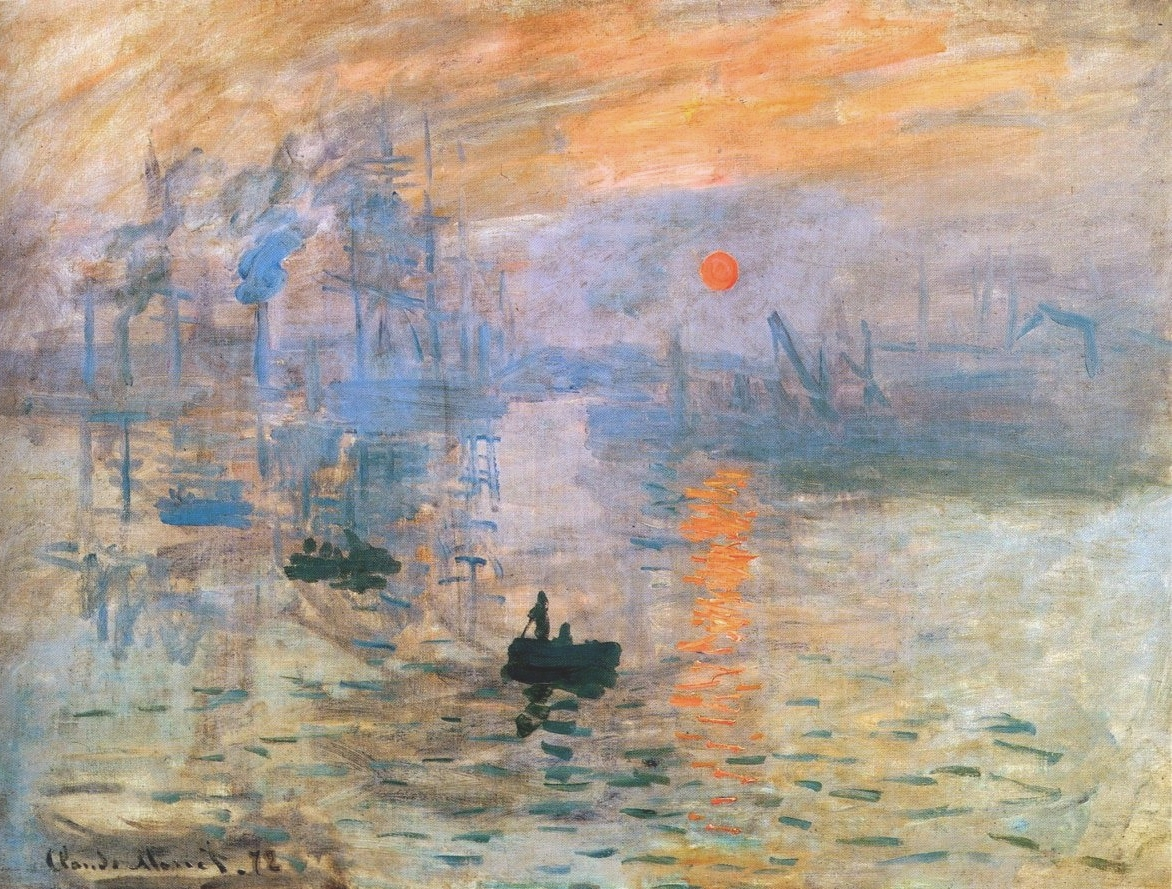
\includegraphics[width=\paperwidth,height=\paperheight]{images/background_image.jpg}% ¡Asegúrate de que este es el nombre correcto de tu imagen!
        }%
    }

    \centering % Centra todo el contenido de la portada

    \vspace*{1.5in} % Ajusta el espacio desde la parte superior (probablemente un poco más que 1in)

    % Título de la tesis: Más grande, negrita y mayúsculas
    {\fontsize{30}{35}\selectfont \textbf{\thesisTitle}} \par
    \vspace{1cm} % Espacio después del título (ajustado de 1.5cm a 1cm)

    % Autor: Grande
    {\Large \authorName} \par
    \vspace{0.7cm} % Espacio después del autor (ajustado de 1cm a 0.7cm)

    % Asesor: Tamaño normal
    {\large Advisor} \par
    {\advisorName} \par  
    \vspace{0.7cm} % Espacio después del asesor (ajustado de 1cm a 0.7cm)

    % Master Thesis
    {\large Master Thesis} \par
    \vspace{0.3cm} % Espacio más pequeño

    % Grado obtenido
    {\large Dissertation presented for the degree of\\ \degreeGranted} \par
    \vspace{0.3cm} % Espacio más pequeño

    % Materia
    {\large In the subject of\\ \subjectField} \par

    \vfill % Empuja la información de la universidad hacia la parte inferior

    % Información de la universidad: Mantenemos el mismo tamaño
    {\large \departmentName \\ \facultyName \\ \universityName} \par
    \vspace{0.5cm} % Espacio después de la universidad (mantenido)

    % Fecha: Mantenemos el mismo tamaño
    {\large \thesisDate} \par
    \vspace{0.5cm} % Espacio después de la fecha para que no quede pegada al borde

\end{titlepage}

\ClearShipoutPictureBG % Limpia el fondo para las páginas siguientes
\clearpage % Fuerza una nueva página
\null\thispagestyle{empty}\newpage

% sections/cover_picture_citation.tex
\thispagestyle{empty} % No mostrar número de página en esta página

\vspace*{\fill} % Empuja el contenido hacia el centro verticalmente

\begin{center}
  {\footnotesize % O \small para una fuente un poco más grande si es necesario
    Cover picture: \textit{"Impression, Sunrise"}, by Claude Monet.
    }  
\end{center}

\clearpage % Fuerza una nueva página después de esta cita


\null\thispagestyle{empty}\newpage

% --- Secciones Preliminares (con numeración romana y sin capítulo) ---
\frontmatter

% --- Dedicación ---
\thispagestyle{empty}

\vspace*{\fill}
\begin{flushright}

\textit{Una palabra escrita es la más selecta de las reliquias.\\
Es algo a la vez más intimo y universal para nosotros \\
que cualquier otra obra de arte pues es, entre ellas,\\ 
la más próxima a la vida misma.\\}

Henry David Thoreau

\vspace{0.5cm}

\textit{Cada obsesión nos convierte en monstruos...}

G. Gospodinov



\end{flushright}

\vspace*{\fill}
\clearpage
\null\thispagestyle{empty}\newpage

% Agradecimientos
% sections/acknowledgements.tex
\cleardoublepage % Asegura que los agradecimientos comiencen en una nueva página (generalmente impar)
\thispagestyle{empty} % Opcional: para que esta página no tenga número de página (la frontmatter los tiene en romano)

\chapter*{Acknowledgements} % <--- CAMBIA ESTO: Define "Acknowledgements" como un capítulo sin numerar
\addcontentsline{toc}{chapter}{Acknowledgements} % <--- Añade esto para que aparezca en el Índice de Contenido




\null\thispagestyle{empty}\newpage

% Abstract
\chapter*{Abstract}
\addcontentsline{toc}{chapter}{Abstract} % Añade "Abstract" a la Tabla de Contenido
This is where English abstract will go.


% Resumen (Español)
\chapter*{Resumen}
\addcontentsline{toc}{chapter}{Resumen} % Añade "Resumen" a la Tabla de Contenido
Aquí va el resumen en español. Debe ser una traducción o adaptación del Abstract.
\null\thispagestyle{empty}\newpage

% Índice de Contenido
\dominitoc % Prepara los mini-índices por capítulo (minitoc); debe ir antes del índice
\tableofcontents


% Lista de Figuras
\listoffigures

% Lista de Tablas
\listoftables

% Notaciones y acrónimos (estilo Del Valle: justo antes del cuerpo principal)
% sections/notations.tex
% --- NOTACIONES Y ACRÓNIMOS (estilo Del Valle) ---
% Del Valle estructura esta sección en dos bloques:
%   1) "Notaciones": prosa que fija las convenciones de símbolos y unidades.
%   2) "Lista de acrónimos": listado a dos columnas (sigla -- significado).
% EDITA el contenido para que refleje las convenciones reales de tu tesis.

\chapter*{Notaciones y acrónimos}
\addcontentsline{toc}{chapter}{Notaciones y acrónimos}
\markboth{Notaciones y acrónimos}{Notaciones y acrónimos}

\section*{Notaciones}

A lo largo del texto se adopta el sistema de unidades $\hbar = 1$, de modo que
energía y frecuencia se expresan en las mismas unidades. % <-- AJUSTA si no aplica a tu caso.
Los operadores se denotan con un acento circunflejo ($\hat{a}$, $\hat{\sigma}$),
y su valor esperado se escribe $\langle \hat{a} \rangle$. Se emplea la notación
habitual de la teoría de conjuntos: $\mathbb{R}$ para los números reales y
$\mathbb{C}$ para los complejos. Los vectores y matrices se escriben en negrita
($\mathbf{x}$, $\mathbf{W}$), y la transpuesta se indica con el superíndice
$^{\mathsf{T}}$.
% AÑADE aquí cualquier otra convención propia de tu trabajo
% (parámetros del láser, hiperparámetros del modelo de aprendizaje, etc.).

\section*{Lista de acrónimos}

\begin{multicols}{2}
\noindent
\begin{description}[leftmargin=5.5em,labelwidth=5em,itemsep=2pt,parsep=0pt]
  \item[\textbf{ML}]   Aprendizaje automático (\textit{Machine Learning})
  \item[\textbf{RL}]   Aprendizaje por refuerzo (\textit{Reinforcement Learning})
  \item[\textbf{NN}]   Red neuronal (\textit{Neural Network})
  \item[\textbf{CNN}]  Red neuronal convolucional
  \item[\textbf{PSO}]  Optimización por enjambre de partículas
  \item[\textbf{GA}]   Algoritmo genético
  \item[\textbf{EA}]   Algoritmo evolutivo
  \item[\textbf{MSE}]  Error cuadrático medio
  \item[\textbf{CW}]   Onda continua (\textit{Continuous Wave})
  \item[\textbf{KLM}]  Anclaje de modos por lente Kerr
  \item[\textbf{SAM}]  Espejo absorbente saturable
  \item[\textbf{SESAM}] Espejo absorbente saturable semiconductor
  \item[\textbf{GVD}]  Dispersión de velocidad de grupo
  \item[\textbf{SPM}]  Automodulación de fase
  \item[\textbf{FWHM}] Anchura a media altura
  \item[\textbf{ODE}]  Ecuación diferencial ordinaria
\end{description}
\end{multicols}

\cleardoublepage

% --- Cuerpo Principal de la Tesis (con numeración arábiga y capítulos) ---
\mainmatter

\chapter{Introducción}
\label{ch:introduccion}
\chapterminitoc

% El presente capítulo establece los fundamentos físicos que rigen la dinámica de los
% pulsos láser ultrarrápidos. A partir de estos conceptos, se formaliza el problema de optimi-
% zación multidimensional inherente al control coherente de dichos pulsos. Finalmente, se
% introduce el aprendizaje automático (machine learning) como un marco computacional
% avanzado para abordar esta complejidad, ofreciendo una perspectiva actualizada del estado
% del arte. Este documento forma parte de un artículo de revisión actualmente en preparación.

Esta tesis estudia cómo optimizar de manera automática los parámetros de un láser ultrarrápido para que genere el pulso deseado. El presente capítulo enmarca ese problema y delimita el trabajo. Comienza situando a los láseres ultrarrápidos y su relevancia científica y tecnológica; muestra a continuación por qué controlar el pulso equivale a resolver un problema de optimización de alta dimensión que los métodos de ajuste tradicionales no afrontan de manera satisfactoria; y, sobre ese diagnóstico, formula la pregunta de investigación, los objetivos, las hipótesis y el alcance del estudio, así como el aporte que la tesis realiza al campo. El tratamiento es deliberadamente conceptual: los fundamentos físicos y computacionales que sostienen el argumento se desarrollan con detalle en el marco teórico (Capítulo~\ref{ch:Theoretical background}). El capítulo concluye con un mapa de lectura del resto del documento.

\section{Contexto y relevancia de los láseres ultrarrápidos}
\label{sec:contexto-relevancia}
 
Pocos instrumentos han ampliado tanto el horizonte de lo observable como el láser ultrarrápido. Su rasgo definitorio es la brevedad: emite pulsos de luz cuya duración se mide en femtosegundos ($10^{-15}$~s) e incluso en attosegundos ($10^{-18}$~s), escalas tan ajenas a la experiencia cotidiana que la proporción entre un attosegundo y un segundo es comparable a la que existe entre un segundo y la edad del universo. Esa brevedad es justamente lo que los hace valiosos: un pulso más corto que el tiempo característico de un proceso permite congelarlo y seguirlo, de modo que la dinámica de electrones, átomos y moléculas (antes inaccesible por ser demasiado rápida) queda al alcance de la medición directa. La Figura~\ref{fig:escala-tiempo} sitúa estas escalas temporales junto con los procesos físicos y las técnicas láser asociadas a cada una.

\begin{figure}[t]
  \centering
  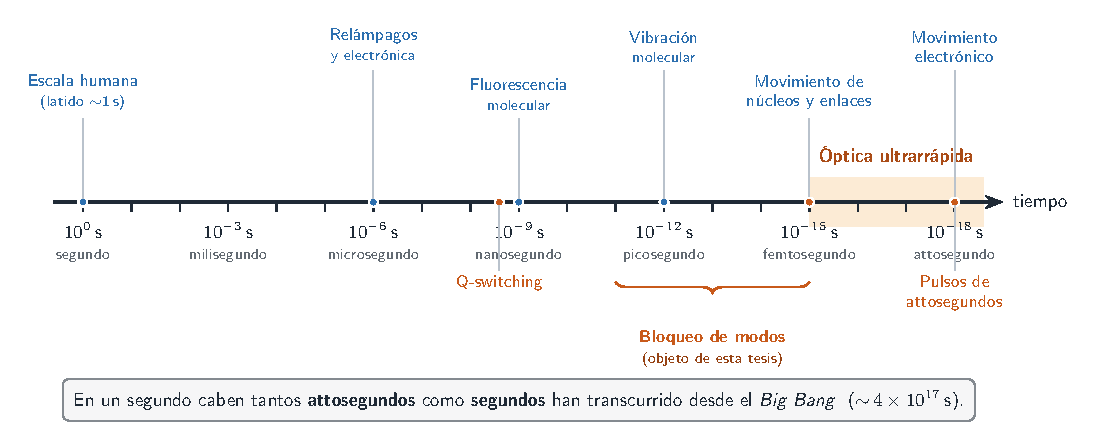
\includegraphics[width=\textwidth]{chapters/images/ch1/fig_escala_tiempo.pdf}
  \caption[Escala de tiempos de la física ultrarrápida]{Escala de tiempos de la
    física ultrarrápida, en eje logarítmico. Sobre el eje se señalan procesos
    físicos característicos de cada escala —desde la escala humana hasta el
    movimiento electrónico— y, bajo él, las técnicas de generación de pulsos
    láser: el \emph{Q-switching}, el bloqueo de modos (objeto de esta tesis) y la
    generación de pulsos de attosegundos. La ventana de la óptica ultrarrápida,
    entre femtosegundos y attosegundos, aparece resaltada.}
  \label{fig:escala-tiempo}
\end{figure}
  
La madurez e impacto de este campo quedaron consagrados con el Premio Nobel de Física de 2023, otorgado a Pierre Agostini, Ferenc Krausz y Anne L'Huillier por el desarrollo de métodos experimentales capaces de generar pulsos de luz de attosegundos, un hito que abrió la puerta a observar el movimiento de los electrones dentro de la materia \cite{Nobel2023}. Ese reconocimiento corona una trayectoria de varias décadas de progreso en la generación y el control de pulsos cada vez más breves e intensos, sostenida por avances sucesivos en medios de ganancia de banda ancha y en arquitecturas de oscilador y amplificación \cite{Krausz1992,Keller2022}.
 
El valor de los láseres ultrarrápidos se manifiesta en un abanico de aplicaciones que atraviesa la ciencia y la tecnología. Su resolución temporal extrema los convierte en el estroboscopio de la espectroscopía de bombeo-sonda, con la que se sigue en tiempo real la relajación electrónica y las transiciones de fase ultrarrápidas. Su capacidad de confinar intensidad en volúmenes microscópicos sustenta técnicas de biofotónica como la microscopía de excitación multifotónica, que permite obtener imágenes tridimensionales de tejido vivo. Su amplísimo ancho de banda es la base de los peines de frecuencia ópticos, que enlazan los dominios del tiempo y la frecuencia con precisión metrológica. Y su elevadísima intensidad pico (accesible gracias a la amplificación de pulsos chirpeados \cite{StricklandMourou1985}) habilita desde la física de campos extremos hasta el micromaquinado de materiales en régimen de ablación en frío. La consolidación de fuentes compactas y fiables, en estado sólido y en fibra, ha extendido este repertorio del laboratorio especializado a un número creciente de entornos \cite{FermannHartl2013}.
 
Conviene, sin embargo, no perder de vista de dónde proviene cada uno de esos pulsos. Detrás de toda esta versatilidad hay siempre un oscilador láser: una cavidad en la que el pulso se forma, se moldea y se estabiliza vuelta tras vuelta. Las propiedades que cada aplicación explota (la duración, la energía, la estabilidad del tren de pulsos) no son un dato de partida, sino el resultado de la dinámica interna de esa cavidad y del modo en que se la ajusta. Es ahí, en el gobierno de la cavidad, donde se decide la calidad del pulso, y es ahí donde surge el problema que esta tesis aborda.


\section{El problema del control y la optimización de parámetros}
\label{sec:problema-control}
 
Disponer de una fuente capaz de emitir pulsos ultracortos no equivale, por sí solo, a disponer del pulso que cada aplicación requiere. Encender el oscilador y obtener un tren de pulsos con una duración, una energía y una estabilidad prescritas son dos cosas distintas: lo segundo exige situar la cavidad en un punto de operación muy concreto, definido por el ajuste simultáneo de un conjunto de magnitudes de control. Es en ese tránsito (de la mera capacidad de generar luz pulsada al gobierno fino de sus propiedades) donde aparece el problema que esta tesis aborda.

\begin{figure}[t]
  \centering
  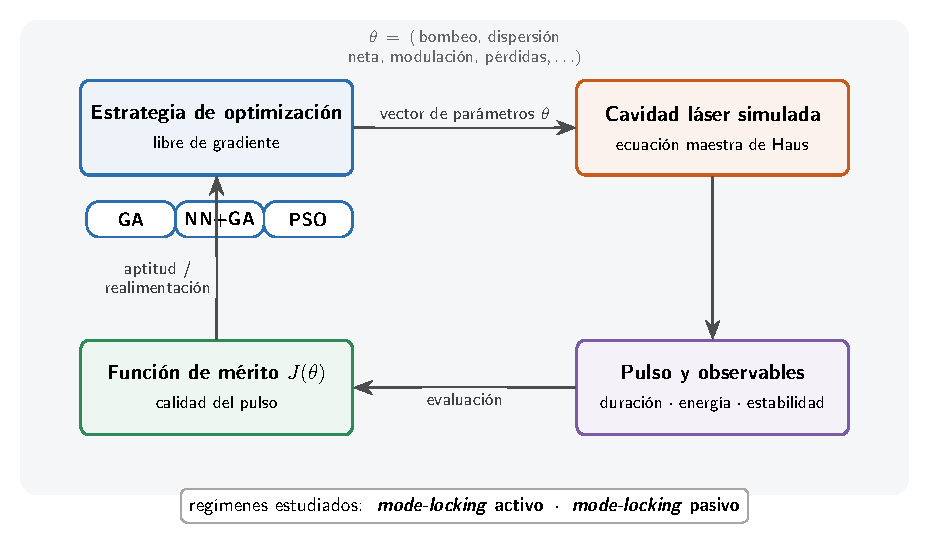
\includegraphics[width=0.92\textwidth]{chapters/images/ch1/fig_esquema_optimizacion.pdf}
  \caption[Ciclo de optimización de la cavidad láser]{Esquema conceptual del
    ciclo de optimización de la cavidad láser. Cada estrategia de optimización
    libre de gradiente (GA, NN+GA o PSO) propone un vector de parámetros
    $\theta$ (bombeo, dispersión neta, modulación, pérdidas, entre otros) que la
    cavidad simulada, modelada por la ecuación maestra de Haus, transforma en un
    pulso. Los observables del pulso (duración, energía y estabilidad) definen la
    función de mérito $J(\theta)$, que realimenta a la estrategia de búsqueda. El
    estudio compara los tres métodos en los regímenes de \emph{mode-locking}
    activo y pasivo.}
  \label{fig:ciclo-optimizacion}
\end{figure}
 
El estado de la cavidad, y con él la existencia misma del pulso y sus características, queda determinado por un puñado de parámetros accesibles al operador: la potencia de bombeo, que fija la ganancia disponible; los parámetros del elemento que produce el anclaje de modos (profundidad y frecuencia de modulación en el régimen activo, profundidad de modulación y tiempo de relajación del absorbente saturable en el pasivo); la dispersión intracavidad neta; el ancho de banda del filtrado espectral; y el acoplamiento de salida, entre otros \cite{Haus2000,Keller2022}. Gobernar el pulso equivale, así, a elegir un punto dentro de un espacio de parámetros de varias dimensiones. La pregunta operativa de toda la tesis puede enunciarse en estos términos: ¿qué combinación de esos valores produce el pulso deseado?
 
La dificultad no reside en el número de variables, sino en que no son independientes. El pulso \emph{mode-locked} es el resultado de un equilibrio delicado entre efectos físicos opuestos (dispersión frente a no linealidad, ganancia frente a pérdidas), de modo que perturbar un solo parámetro rompe ese equilibrio y obliga a reajustar los demás para preservar la estabilidad del pulso. El sistema no admite, por tanto, una optimización variable por variable: los grados de libertad están acoplados, y el efecto de cada uno depende del valor de todos los otros. La descripción formal de ese acoplamiento (la dinámica de la envolvente en la cavidad y el balance que sostiene al pulso) corresponde al marco teórico y se desarrolla en el Capítulo~\ref{ch:Theoretical background}; aquí basta con retener su consecuencia: el ajuste es un problema global, no una suma de ajustes locales.
 
Ese acoplamiento dota al espacio de búsqueda de una estructura particularmente hostil. Es un espacio de \emph{alta dimensión}, en el que el volumen a explorar crece de forma explosiva con cada grado de libertad añadido; es \emph{no convexo}, poblado de óptimos locales en los que los métodos basados en gradiente quedan atrapados; y es \emph{multiestable}, en el sentido de que para un mismo conjunto de parámetros pueden coexistir varios regímenes de operación estables (onda continua, anclaje fundamental y armónico, regímenes multipulso o de \emph{Q-switching}), de manera que el estado finalmente alcanzado depende no solo de dónde se está en el espacio, sino del camino por el que se llegó \cite{Andral2015,GreluAkhmediev2012,Kokhanovskiy2022}. A ello se añaden las transiciones abruptas entre regímenes y el ruido inherente a cualquier oscilador real, que exigen que una solución útil no sea solo óptima en un punto, sino además robusta frente a perturbaciones.
 
El cuadro resultante es el de un problema de optimización de caja negra: no se dispone de una expresión cerrada que relacione los parámetros con la calidad del pulso, cada evaluación obliga a propagar el estado de la cavidad hasta su régimen estacionario, y el paisaje de búsqueda carece de la regularidad que los métodos analíticos requieren \cite{Genty2021,Woodward2016}. Optimizar un láser ultrarrápido es, en definitiva, un problema de búsqueda en un espacio difícil, no un cálculo que pueda resolverse de forma cerrada. Este es el obstáculo central que motiva la presente tesis; antes de presentar las estrategias que la comunidad ha desarrollado para sortearlo, conviene examinar por qué los enfoques de ajuste tradicionales resultan insuficientes frente a un espacio con estas características. La Figura~\ref{fig:ciclo-optimizacion} resume el ciclo de optimización que de aquí resulta y que esta tesis aborda: una estrategia de búsqueda —en este trabajo, el algoritmo genético (GA), su acoplamiento con una red neuronal (NN+GA) y la optimización por enjambre de partículas (PSO)— propone vectores de parámetros que la cavidad simulada convierte en pulsos, cuya calidad, cuantificada por una función de mérito, realimenta la búsqueda.


\section{Limitaciones de los enfoques tradicionales de ajuste}
\label{sec:enfoques-tradicionales-intro}
 
Frente a un espacio de búsqueda con las características descritas, las estrategias con que tradicionalmente se ha ajustado un láser \emph{mode-locked} resultan insuficientes, cada una por una razón distinta. El enfoque históricamente dominante ha sido el \emph{ajuste manual experto}: un operador modifica iterativamente los parámetros accesibles mientras vigila la traza temporal y el espectro, guiándose por heurísticas adquiridas con la práctica. Su fortaleza es la intuición acumulada, pero sus límites son estructurales: es lento, porque explora el espacio punto a punto; es poco reproducible, porque el resultado depende del operador; no escala con la dimensión; y no ofrece recuperación automática cuando la deriva ambiental saca al láser de su régimen \cite{Pu2019,Pu2020}.
 
La alternativa de fuerza bruta (el \emph{barrido exhaustivo} del espacio de parámetros) garantiza cobertura y reproducibilidad, pero choca con la maldición de la dimensión: el número de evaluaciones crece exponencialmente y, como cada una exige llevar la cavidad a su estado estacionario, el costo se vuelve prohibitivo ya para pocas variables \cite{Andral2015}. El \emph{diseño analítico} basado en la teoría de cavidad ofrece, por su parte, leyes de escala y valores de partida útiles, pero su validez descansa en aproximaciones que eluden justamente los fenómenos que dominan el problema real (multiestabilidad, transiciones abruptas y ruido), de modo que entrega un buen punto inicial, no una solución en lazo cerrado. Y los métodos de \emph{control clásico} y de \emph{optimización basada en gradiente} presuponen una respuesta suave y diferenciable entre la acción y el observable, hipótesis que una cavidad multiestable e histerética incumple de raíz \cite{Kokhanovskiy2022}.
 
El denominador común es que ninguno de estos enfoques afronta de manera conjunta las dificultades del problema: explorar globalmente un espacio de alta dimensión y no convexo, tolerar su naturaleza de caja negra y discontinua, y operar de forma autónoma y robusta frente al ruido. Es precisamente esa carencia simultánea la que define el nicho ocupado, en la última década, por los algoritmos de optimización inspirados en la naturaleza y las técnicas de aprendizaje automático \cite{Genty2021}: métodos que no exigen gradientes, exploran soluciones en paralelo y se prestan a automatizar el ciclo completo de ajuste. La revisión sistemática de cómo el campo ha desplegado esas herramientas (y de las brechas que deja abiertas) constituye el Estado del Arte que se presenta en el Capítulo~\ref{ch:estado del arte}.


\section{Planteamiento del problema y pregunta de investigación}
\label{sec:planteamiento}
 
Las secciones anteriores permiten enunciar el problema con precisión. Generar el pulso que una aplicación requiere equivale a fijar la configuración de parámetros de un oscilador láser, y ese ajuste constituye un problema de optimización de caja negra (de alta dimensión, no convexo, multiestable y ruidoso) frente al cual los enfoques tradicionales de ajuste resultan insuficientes. La comunidad ha respondido adoptando algoritmos de optimización inspirados en la naturaleza y técnicas de aprendizaje automático, capaces de explorar globalmente el espacio sin exigir gradientes ni un modelo analítico de la respuesta de la cavidad. Sin embargo, como se documenta en el Estado del Arte (Capítulo~\ref{ch:estado del arte}), ese cuerpo de trabajo deja dos vacíos persistentes: por un lado, la optimización automatizada se ha concentrado casi por completo en el \emph{mode-locking} pasivo, dejando el régimen activo notablemente subexplorado \cite{KuizengaSiegman1970}; por otro, la literatura está organizada como una colección de estudios de caso aislados, sin comparaciones sistemáticas que mantengan fijos el láser, el espacio de parámetros y la función objetivo para variar únicamente el algoritmo \cite{Genty2021,Jiang2022}.
 
De esos dos vacíos surge la pregunta que vertebra esta tesis: \emph{¿cómo se comparan tres estrategias de optimización inspiradas en la naturaleza (el algoritmo genético (GA), una red neuronal acoplada al algoritmo genético como sustituto del simulador (NN+GA) y la optimización por enjambre de partículas (PSO)) al ajustar los parámetros de una cavidad láser ultrarrápida, evaluadas bajo idénticas condiciones de simulación numérica y en los regímenes de} mode-locking \emph{tanto activo como pasivo?} La pregunta se descompone en tres interrogantes operativos: qué calidad de pulso alcanza cada método respecto a una misma función de mérito; a qué costo computacional lo hace (en número de evaluaciones del simulador y en tiempo hasta la convergencia); y con qué robustez reproduce su desempeño al variar las condiciones iniciales y la modalidad de anclaje.
 
El interés de la pregunta no es solo práctico sino metodológico. Las tres estrategias comparten el paradigma de la optimización libre de gradiente, pero difieren de manera controlada en la mecánica de búsqueda y en el modo de evaluar la función objetivo, de suerte que confrontarlas sobre un mismo banco de pruebas permite atribuir las diferencias de rendimiento al método y no a las particularidades del problema. Responderla, además, sobre las dos modalidades de \emph{mode-locking} aborda simultáneamente las dos brechas señaladas. Los objetivos que concretan esta pregunta en entregables verificables se enuncian a continuación.


\section{Objetivos}
\label{sec:objetivos}
 
\subsection*{Objetivo general}
 
Comparar de forma sistemática tres estrategias de optimización inspiradas en la naturaleza (el algoritmo genético (GA), una red neuronal acoplada al algoritmo genético como sustituto del simulador (NN+GA) y la optimización por enjambre de partículas (PSO)) en el ajuste de los parámetros de una cavidad láser ultrarrápida simulada numéricamente, evaluándolas bajo idénticas condiciones en los regímenes de \emph{mode-locking} activo y pasivo.
 
\subsection*{Objetivos específicos}
 
\begin{enumerate}
  \item Implementar un modelo numérico de la cavidad láser, basado en la ecuación maestra de Haus, capaz de reproducir los regímenes de operación conocidos y de servir como entorno de evaluación para los algoritmos de optimización.
 
  \item Formular el problema de optimización asociado, definiendo las variables de decisión, sus rangos y restricciones, y una función de mérito que cuantifique la calidad del pulso a partir de observables del estado estacionario de la cavidad.
 
  \item Implementar y ajustar un algoritmo genético sobre ese problema, que sirva como línea base de referencia frente a la cual contrastar las demás estrategias.
 
  \item Construir una red neuronal que actúe como sustituto (\emph{surrogate}) del simulador y acoplarla al algoritmo genético (NN+GA), con el fin de reducir el número de evaluaciones costosas durante la búsqueda.
 
  \item Implementar la optimización por enjambre de partículas sobre el mismo problema, con su propia parametrización del proceso de búsqueda.
 
  \item Comparar los tres métodos en los regímenes de \emph{mode-locking} activo y pasivo bajo un conjunto común de métricas (calidad del pulso, costo computacional y robustez), de modo que las diferencias de desempeño puedan atribuirse al algoritmo y no a las particularidades del problema.
\end{enumerate}
 
Cada objetivo específico se traduce en un componente verificable del trabajo: los dos primeros definen el entorno de simulación y el problema de optimización (Capítulo~\ref{ch:Theoretical background} y Capítulo~\ref{ch:Methodology}); el tercero, el cuarto y el quinto, la implementación de cada método; y el sexto, el estudio comparativo que constituye el aporte central de la tesis y que se desarrolla en los capítulos de metodología y resultados.

 
\section{Hipótesis, alcance y limitaciones}
\label{sec:hipotesis-alcance}
 
La hipótesis de trabajo que orienta este estudio es que las tres estrategias consideradas son capaces de alcanzar soluciones de calidad comparable sobre la misma función de mérito, pero difieren de manera medible en su eficiencia y su comportamiento de búsqueda (en el número de evaluaciones del simulador que requieren, en el tiempo hasta la convergencia y en la robustez de su desempeño), de modo que existe un método preferible según el régimen de \emph{mode-locking} considerado. En particular, se espera que el acoplamiento de la red neuronal como sustituto del simulador (NN+GA) reduzca el costo de evaluación frente al algoritmo genético puro, y que la estructura más determinista y de menor dimensión del régimen activo favorezca una convergencia más rápida que la del régimen pasivo. El estudio comparativo está diseñado para confirmar o refutar estas expectativas sobre una base empírica controlada.
 
El alcance del trabajo queda delimitado por tres decisiones. Primero, el estudio se realiza enteramente en \emph{simulación numérica}: la cavidad se representa mediante el modelo de la ecuación maestra de Haus, que actúa como entorno de evaluación para los optimizadores. Segundo, la comparación abarca las dos modalidades de \emph{mode-locking}, activa y pasiva, y se restringe a las tres estrategias seleccionadas (GA, NN+GA y PSO), elegidas por compartir el paradigma de la optimización libre de gradiente y diferir de forma controlada en la mecánica de búsqueda. Tercero, la calidad de las soluciones se mide mediante una función de mérito definida sobre observables del pulso (duración, energía y estabilidad) en el estado estacionario de la cavidad.
 
De ese alcance se derivan sus limitaciones, que conviene reconocer explícitamente. Al emplear simulación pura como generador de datos, los resultados no incorporan de forma plena el ruido, la deriva de parámetros y las no idealidades presentes en un montaje experimental, por lo que sus conclusiones se circunscriben al modelo y no se extrapolan sin más a un laboratorio \cite{Baumeister2018}. Del mismo modo, el desempeño observado depende del modelo de cavidad adoptado y de los rangos de parámetros explorados, cuya elección acota el espacio de búsqueda. Finalmente, el trabajo se concentra en la familia de optimizadores libres de gradiente y deja fuera de su foco comparativo el aprendizaje por refuerzo profundo, que —pese a su potencial para el control de la multiestabilidad \cite{Kokhanovskiy2024}— se considera un horizonte de extensión y no parte del estudio comparativo. Estas limitaciones no debilitan el aporte: lo delimitan con honestidad y orientan la interpretación de los resultados.

\section{Aporte de la tesis}
\label{sec:aporte}
 
La contribución de esta tesis se define por las dos brechas que el Estado del Arte deja al descubierto y que el trabajo aborda de manera conjunta en un único diseño experimental. La primera es una brecha de \emph{objeto}. La optimización automatizada de láseres \emph{mode-locked} se ha desarrollado casi exclusivamente sobre el régimen pasivo, dejando el \emph{mode-locking} activo notablemente subexplorado como problema de ajuste inteligente \cite{Woodward2016,Andral2015}. Esta tesis amplía ese alcance al aplicar un mismo conjunto de optimizadores a ambas modalidades, lo que permite examinar si las técnicas que han demostrado su eficacia en el régimen pasivo conservan su desempeño cuando se enfrentan a la dinámica más determinista y de menor dimensión del activo.
 
La segunda es una brecha de \emph{método}. La literatura está organizada como una colección de estudios de caso en los que cada trabajo valida un único algoritmo sobre un único problema, lo que impide atribuir limpiamente las diferencias de rendimiento al método empleado \cite{Genty2021}. El aporte de esta tesis es un estudio comparativo controlado de GA, NN+GA y PSO que mantiene fijos el láser, el espacio de parámetros y la función de mérito, y varía únicamente el algoritmo de optimización, de modo que las diferencias observadas reflejen el comportamiento del método y no las particularidades del problema. Atender ambas brechas en un mismo diseño (los tres optimizadores sobre las dos modalidades de anclaje) es lo que distingue a este trabajo de los antecedentes revisados.
 
A esas dos contribuciones se añade un valor metodológico transversal: el estudio se articula como un protocolo comparativo \emph{reproducible}, con un mismo simulador, un mismo conjunto de métricas (calidad del pulso, costo computacional y robustez) y un control explícito de la aleatoriedad y de las repeticiones. Más allá de los resultados concretos que arroje, ese protocolo constituye un marco con el que futuros métodos de optimización podrán evaluarse sobre una base común, lo que responde directamente a la fragmentación que caracteriza al campo.


\section{Resumen de contenido}
\label{sec:estructura-documento}
 
El resto de la tesis sigue el mismo hilo conductor que esta introducción, avanzando de la caracterización del problema a su resolución y a la interpretación de los resultados. El Capítulo~\ref{ch:estado del arte} presenta el estado del arte: revisa la literatura sobre optimización de láseres ultrarrápidos siguiendo un recorrido que va de la física de la cavidad a las estrategias computacionales, y justifica, sobre esa base, las dos brechas que el trabajo se propone llenar. El Capítulo~\ref{ch:Theoretical background} desarrolla el marco teórico, reuniendo las herramientas físicas y computacionales necesarias para el resto del documento: la dinámica de la cavidad y la ecuación maestra de Haus, los regímenes de \emph{mode-locking} activo y pasivo, y los fundamentos de las tres estrategias de optimización.
 
El Capítulo~\ref{ch:Methodology} expone la metodología del estudio comparativo: el modelo numérico de la cavidad, la definición del problema de optimización y de la función de mérito, la implementación de cada método y el diseño del experimento que los enfrenta bajo idénticas condiciones. El capítulo de resultados presenta los hallazgos (la validación del modelo y el desempeño de cada estrategia en ambas modalidades de anclaje) sin interpretarlos todavía. El capítulo de discusión da sentido a esos resultados, interpreta físicamente las soluciones halladas, contrasta las fortalezas y debilidades de cada método y dialoga con la literatura revisada. Finalmente, el capítulo de conclusiones cierra el círculo abierto en esta introducción: responde a la pregunta de investigación, recapitula las contribuciones y señala las líneas de trabajo futuro, entre ellas la validación experimental y la extensión al aprendizaje por refuerzo.
\cleardoublepage

\chapter{Estado del arte}
\label{ch:estado del arte}
\chapterminitoc


Este capítulo revisa el cuerpo de literatura sobre el que se asienta la presente tesis y construye, a partir de él, la justificación de su contribución. La revisión sigue un único hilo conductor que va de la física al control: comienza por el objeto físico que se quiere gobernar —el pulso ultracorto y la dinámica disipativa de la cavidad láser que lo genera— y avanza hasta las estrategias computacionales con que la comunidad ha aprendido a ajustar ese sistema de forma automática. En consecuencia, se organiza en tres partes encadenadas. La primera parte establece los fundamentos físicos en el marco de modelado de cavidad de Keller y Krausz: la generación y propagación de pulsos ultracortos, el \emph{mode-locking} entendido como un sistema dinámico disipativo, la estructura del espacio de parámetros que de allí resulta y las limitaciones de los enfoques de ajuste tradicionales. La segunda parte reconstruye, en orden histórico y metodológico, cómo el aprendizaje automático y la optimización inspirada en la naturaleza han ocupado ese terreno —del control adaptativo \emph{data-driven} a los algoritmos evolutivos, las redes neuronales y el aprendizaje por refuerzo—, mostrando que cada familia surgió para corregir una limitación de la anterior. La tercera parte, por último, identifica las dos brechas que esta revisión deja al descubierto )(el predominio del \emph{mode-locking} pasivo y la ausencia de comparaciones sistemáticas entre métodos) y posiciona la tesis como respuesta a ambas, antes de sintetizar el recorrido completo.

\section{Pulsos ultracortos: generación y propagación}
\label{sec:pulsos-ultracortos}
La optimización automatizada de los parámetros de un láser ultrarrápido requiere una comprensión rigurosa de los mecanismos físicos subyacentes. Las dificultades operativas que justifican el uso del aprendizaje automático en este ámbito no constituyen contingencias de ingeniería, sino consecuencias directas de la compleja física no lineal que rige la dinámica del pulso. El presente apartado examina el proceso de formación y estabilización de estos paquetes ópticos de extrema brevedad durante su propagación intracavidad. Esta revisión se fundamenta en la literatura seminal y en síntesis contemporáneas, enmarcándose en la tradición del modelado de cavidades establecida por Keller y Krausz \cite{Keller2022, Krausz1992}.

El régimen ultrarrápido se caracteriza por duraciones de pulso inferiores al picosegundo ($1 ps = 10^{-12}$ s) y, en su límite fundamental, cercanas a escasos ciclos del campo eléctrico, en el orden de los femtosegundos (1 fs $= 10^-15$ s). Esta severa confinación temporal impone dos propiedades físicas insoslayables. En primer lugar, de acuerdo con la relación de incertidumbre tiempo-frecuencia, la brevedad temporal exige un ancho de banda espectral extenso; en consecuencia, el pulso debe modelarse matemáticamente como un paquete de ondas y no como una onda monocromática \cite{Keller2022}. En segundo lugar, la concentración de la energía óptica en una ventana temporal mínima incrementa drásticamente la potencia pico. Esto induce una propagación fuertemente no lineal incluso para energías por pulso moderadas \cite{Agrawal2019}. Ambos factores determinan la evolución espaciotemporal del pulso, activando mecanismos que, de operar aisladamente, inducirían la desintegración del paquete de ondas.

La extensa amplitud espectral exacerba los efectos de la dispersión de la velocidad de grupo (GVD). Dado que las distintas componentes espectrales viajan a diferentes velocidades, el pulso experimenta un ensanchamiento dispersivo conforme se propaga a través de los elementos intracavidad, perdiendo el confinamiento temporal que lo define. Simultáneamente, la elevada intensidad pico activa el efecto Kerr óptico: el índice de refracción del medio intracavidad deja de ser lineal y pasa a depender de la intensidad instantánea, modelado como $n(I) = n_0 + n_2 I$ \cite{Agrawal2019}. El pulso induce entonces una automodulación de fase (SPM) (fenómeno observado tempranamente en fibras de sílice por Stolen y Lin \cite{StolenLin1978}) lo que genera nuevas componentes frecuenciales y ensancha el espectro con un chirp de frecuencia aproximadamente lineal en su región central. Aunque ambos efectos parecen disruptivos por separado (uno dispersa el pulso en el tiempo, el otro lo deforma en frecuencia), la síntesis cuantitativa de su interacción sobre la envolvente de variación lenta del campo eléctrico $A(z,T)$ se describe mediante la ecuación de Schrödinger no lineal (NLSE) \cite{Agrawal2019}:

\begin{equation}
  \frac{\partial A}{\partial z} + \frac{i\beta_2}{2}\frac{\partial^2 A}{\partial T^2} = i\gamma|A|^2 A  
\end{equation}

donde $\beta_2$ representa el parámetro de GVD y $\gamma$ es el coeficiente no lineal. En un resonador láser, esta ecuación diferencial se integra junto con términos de ganancia, pérdidas y mecanismos de saturación en el marco de una ecuación maestra (discutida en detalle en la Sección \ref{sec:mode-locking}). No obstante, es la convergencia de la dispersión y la no linealidad en el marco de la NLSE lo que revela dinámicas emergentes imposibles de deducir de forma aislada.

El corolario analítico más notable de esta interacción es el solitón óptico. Hasegawa y Tappert demostraron teóricamente que, en el régimen de dispersión anómala ($\beta_2 < 0$), el ensanchamiento dispersivo y el desplazamiento de fase inducido por SPM pueden compensarse de forma exacta, permitiendo la propagación invariante del pulso \cite{HasegawaTappert1973}; un fenómeno que Mollenauer et al. verificaron experimentalmente en fibras ópticas pocos años después \cite{Mollenauer1980}. Así, la interacción de dos fenómenos aparentemente disruptivos establece una condición de estabilidad morfológica. Sin embargo, la extrapolación de este concepto a la dinámica de una cavidad láser exige considerar la naturaleza no conservativa del sistema (presencia de ganancia, atenuación y filtrado espectral). En este contexto emerge el solitón disipativo, una estructura autoorganizada que se sostiene mediante un doble equilibrio dinámico: dispersión frente a no linealidad, y ganancia óptica frente a pérdidas \cite{GreluAkhmediev2012}. Esta noción constituye el eje articulador del presente trabajo: el pulso en régimen de mode-locking que los algoritmos buscarán estabilizar es, fundamentalmente, un solitón disipativo. Su existencia depende de una calibración milimétrica de los parámetros de la cavidad, dinámica que se fundamenta en las formulaciones teóricas canónicas de Haus \cite{Haus2000} y cuyo modelado como sistema dinámico se aborda en la Sección \ref{sec:mode-locking}.

El salto tecnológico decisivo para el desarrollo de fuentes ultrarrápidas de alta potencia fue la técnica de amplificación de pulsos chirpeados (CPA), concebida por Strickland y Mourou \cite{StricklandMourou1985}. Esta arquitectura mitiga el daño óptico inducido por las altas intensidades pico estirando temporalmente el pulso previo a su amplificación y recomprimiéndolo posteriormente, logrando así el desacople entre energía total e intensidad pico. Sobre esta base maduraron los osciladores de estado sólido de femtosegundos, un desarrollo ampliamente documentado en las revisiones de Krausz et al. \cite{Krausz1992} y Keller \cite{Keller2022, Keller2003}. En este punto, los fundamentos físicos convergen con el problema de optimización central de esta tesis: la generación autónoma de un pulso ultracorto intracavidad exige equilibrar simultáneamente la dispersión, la no linealidad, la ganancia y las pérdidas. Este frágil equilibrio depende de un vector de parámetros altamente acoplados, cuyo ajuste preciso determina la viabilidad y estabilidad del régimen. Esta extrema sensibilidad paramétrica convierte el control del láser en un problema de optimización multivariable complejo (analizado en la Sección \ref{sec:espacio-parametros}), motivando la adopción de las técnicas de aprendizaje automático evaluadas en la Parte B de esta investigación.

\section{El mode-locking como sistema dinámico disipativo}
\label{sec:mode-locking}

Habiéndose establecido los mecanismos de estabilidad temporal y espectral del pulso ultracorto durante su propagación adiabática, resulta fundamental determinar las condiciones físicas bajo las cuales una cavidad láser genera dichos estados de forma espontánea y estacionaria en lugar de emitir en un régimen de onda continua (CW). El bloqueo de modos o \emph{mode-locking} constituye el fenómeno no lineal central objeto de optimización en esta investigación. Su descripción formal como un sistema dinámico disipativo, fundamentada en los modelos de cavidad pioneros de Keller y Krausz \cite{Krausz1992,Keller2022}, proporciona el marco analítico necesario para abordar el problema de control óptimo. Cabe precisar que el dominio físico de este trabajo se circunscribe rigurosamente a la dinámica global de la cavidad resonantemente acoplada, abstrayéndose de la consideración de la fibra óptica exclusivamente como una guía de onda pasiva.

Etimológicamente, el fenómeno se describió inicialmente en el dominio de la frecuencia. Una cavidad láser convencional alberga un espectro discreto de modos longitudinales equidistantes; si estos modos oscilan con fases estocásticamente independientes, su interferencia aleatoria produce una emisión cuasi-continua caracterizada por intensas fluctuaciones de ruido de fase y amplitud. Por el contrario, al inducir una relación de fase fija y constante entre dichos modos, la superposición coherente de los campos eléctricos genera un único pulso de alta intensidad que circula intracavidad. Este paquete de energía se acopla parcialmente al exterior en cada periodo de tránsito temporal, generando un tren periódico de pulsos ultracortos. Si bien esta representación modal es físicamente exacta, carece de la operatividad matemática necesaria para evaluar la estabilidad asintótica y las bifurcaciones dinámicas del pulso frente a perturbaciones. Consiguientemente, el análisis contemporáneo adopta un enfoque formal en el dominio del tiempo, evaluando la evolución iterativa de la envolvente temporal vuelta a vuelta a través de las transformaciones no unitarias operadas por los componentes de la cavidad.

Esta descripción temporal se sustenta en dos hitos teóricos fundamentales. El primero corresponde al análisis del bloqueo de modos activo desarrollado por Kuizenga y Siegman \cite{KuizengaSiegman1970}. Mediante la propagación de un perfil gaussiano elemental bajo una condición de autoconsistencia en un tránsito cerrado, los autores dedujeron expresiones analíticas explícitas para la duración, el \emph{chirp} y el ancho de banda espectral del pulso en presencia de una modulación síncrona externa. Este modelo demostró cuantitativamente que la anchura temporal estacionaria está unívocamente determinada por el equilibrio entre el estrechamiento temporal inducido por el modulador y la limitación espectral impuesta por el ancho de banda finito del medio de ganancia. El segundo hito analítico lo constituye la formulación de la \emph{ecuación maestra} por Haus \cite{Haus1975fast,Haus2000}. Esta aproximación postula una ecuación integro-diferencial de evolución continua para la envolvente lenta del campo, integrando de forma aditiva los efectos discretos distribuidos en una vuelta de cavidad: ganancia con filtrado parabólico, pérdidas lineales, dispersión cromática, no linealidad de fase (efecto Kerr) y la acción de elementos de conmutación óptica. La ecuación maestra de Haus representa el formalismo matemático unificado predominante para describir regímenes tanto activos como pasivos, sirviendo de núcleo estructural para el modelo numérico de la presente investigación.

Dentro de este marco conceptual, la clasificación fundamental radica en la naturaleza del mecanismo de modulación. El bloqueo de modos activo emplea un dispositivo externo (un modulador electro-óptico o acusto-óptico) sincronizado con el tiempo de tránsito de la cavidad. Este introduce una modulación de pérdidas periódica que discrimina selectivamente la radiación, favoreciendo el crecimiento del campo óptico localizado en el mínimo de pérdidas y comprimiéndolo progresivamente en un pulso solitario, conforme a la teoría del anclaje forzado de Haus \cite{Haus1975forced} y los formalismos previamente citados \cite{KuizengaSiegman1970}. Por el contrario, el bloqueo de modos pasivo prescinde de señales de reloj externas, implementando un absorbente saturable cuya atenuación disminuye de forma no lineal en función de la intensidad instantánea del campo óptico. En este régimen autoinducido, el propio pulso genera dinámicamente la ventana temporal de baja pérdida que promueve su amplificación. La cinética de este proceso varía críticamente dependiendo de si el tiempo de relajación del absorbente es rápido o lento en comparación con la duración del pulso, escenarios analizados formalmente por Haus \cite{Haus1975fast,Haus2000}. La realización experimental de este principio físico en osciladores de estado sólido (mediante reflectores de absorbente saturable semiconductor (SESAM) \cite{Keller1996} o mediante el efecto de lente de Kerr (\emph{Kerr-lens mode-locking}, KLM) \cite{Krausz1992}) permitió alcanzar el régimen de pocos ciclos ópticos, consolidando la tecnología ultrarrápida moderna \cite{Keller2003,Keller2022}. Esta asimetría mecanística reviste una relevancia metodológica crucial: como se detallará más adelante, la literatura científica sobre optimización automatizada se ha focalizado casi exclusivamente en configuraciones pasivas debido a su inherente complejidad paramétrica, dejando el régimen activo sustancialmente inexplorado en el ámbito del control óptimo adaptativo.

La convergencia analítica entre ambas modalidades, que justifica la aplicación de metodologías de optimización análogas, reside en caracterizar la cavidad láser como un sistema dinámico disipativo no lineal guiado contractivamente por un flujo continuo de energía. El sistema experimenta un aporte energético constante a través del bombeo óptico y una disipación sistemática mediada por pérdidas internas y el acoplamiento de salida; en este contexto, el pulso estacionario emerge como una estructura disipativa autoorganizada. Por consiguiente, el pulso en régimen de \emph{mode-locking} no se comporta como una solución solitaria conservativa —característica de la NLSE ideal analizada en la Sección \ref{sec:pulsos-ultracortos}—, sino como un \emph{solitón disipativo}: un atractor de base compacta en el espacio de fases, sustentado por el equilibrio simultáneo en los balances acoplados de dispersión-no linealidad y ganancia-pérdida \cite{GreluAkhmediev2012}. Esta perspectiva topológica impone dos implicaciones fenomenológicas cardinales para este estudio. En primer lugar, al tratarse de un sistema no lineal disipativo de alta dimensionalidad, la cavidad exhibe una marcada multiestabilidad, coexistiendo una pluralidad de atractores estables para un mismo conjunto de parámetros —tales como el régimen de onda continua, el bloqueo de modos fundamental, estados armónicos, multipulsos cooperativos o regímenes de inestabilidad tipo \emph{Q-switching}— \cite{Akhmediev2005}. En consecuencia, el estado asintótico del sistema muestra una estricta dependencia de la trayectoria histórica y de las condiciones iniciales (histéresis). En segundo lugar, el atractor específico alcanzado y sus métricas de calidad físico-óptica dependen de forma extremadamente sensible y no monótona del ajuste de precisión de los parámetros globales de la cavidad. La caracterización rigurosa de este espacio de estados —definido por su alta dimensionalidad, topología no convexa y multiestabilidad intrínseca— constituye el objeto de estudio de la Sección \ref{sec:espacio-parametros}, sirviendo de nexo directo hacia la formulación del problema de optimización mediante algoritmos avanzados.

\section{Espacio de parámetros y estructura del problema de optimización}
\label{sec:espacio-parametros}

Una vez caracterizado el pulso bajo el régimen de bloqueo de modos (\emph{mode-locking}) como un atractor estable dentro de una cavidad disipativa no lineal, resulta imperativo formalizar esta observación fenomenológica bajo el marco riguroso de un problema de optimización matemática. Las restricciones intrínsecas y la topología no trivial de dicho espacio de búsqueda determinan de manera unívoca la complejidad operacional del sistema. Por consiguiente, la implementación de arquitecturas de aprendizaje automático y algoritmos de optimización global analizados adelante no responde a una preferencia metodológica arbitraria, sino a un diagnóstico analítico de la estructura geométrica y dinámica de la hipersuperficie de coste, cuya resolución mediante técnicas de ajuste tradicionales resulta impracticable \cite{Genty2021}.

La formulación analítica del problema requiere la definición formal de un vector de parámetros de control, $\mathbf{p} \in \mathbb{R}^d$, que condense los grados de libertad experimentales accesibles en el sistema. En configuraciones físicas representativas, este vector comprende variables operacionales críticas como la potencia de bombeo óptico (que determina la ganancia saturable disponible), los parámetros específicos del mecanismo de modulación (frecuencia y profundidad de modulación en regímenes activos; profundidad de modulación, umbral de saturación y tiempo de relajación del absorbente saturable en regímenes pasivos), la dispersión cromática neta de la cavidad, el ancho de banda efectivo del filtrado espectral y el coeficiente de acoplamiento de la salida óptica, entre otros \cite{Haus2000,Keller2022}. El espacio objetivo, por su parte, no se restringe a un funcional escalar elemental, sino que describe una condición global de estabilidad asintótica sobre el estado dinámico intracavidad. El propósito matemático consiste en converger de manera robusta hacia un régimen de pulso único y coherente que maximice figuras de mérito específicas —típicamente la energía de pulso o el ancho de banda espectral, minimizando concurrentemente la duración temporal—, al tiempo que se eluden regímenes colaterales degenerados o inestables. La traslación de estas condiciones físicas a una función objetivo numéricamente evaluable a partir de observables experimentales medibles (como trazas de autocorrelación, espectrogramas o perfiles de autocorrelación de intensidad) constituye un desafío metodológico crítico en la literatura contemporánea \cite{Genty2021}.

Las complejidades que restringen y configuran este espacio de búsqueda emanan directamente de la naturaleza no lineal y disipativa del sistema dinámico subyacente. En primer lugar, el problema exhibe una marcada \emph{alta dimensionalidad}: incluso las arquitecturas de cavidad elementales involucran múltiples variables ortogonales fuertemente acopladas entre sí. En sistemas avanzados que incorporan el control activo de la birrefringencia y el estado de polarización no lineal, el número de grados de libertad efectivos crece de forma exponencial, inhabilitando la exploración del espacio mediante barridos paramétricos exhaustivos debido al coste temporal y computacional asociado \cite{Andral2015}. En segundo lugar, el paisaje de la función objetivo se caracteriza por una inherente \emph{no convexidad}. La hipersuperficie de coste carece de un óptimo global unimodal y presenta, en su lugar, una topología irregular y fragmentada con densos óptimos locales y mesetas de gradiente nulo, escenarios donde los algoritmos clásicos de descenso de gradiente convergen de forma prematura o quedan confinados indefinidamente \cite{Boyd2004}. En tercer lugar, la propiedad más disruptiva del sistema radica en la \emph{multiestabilidad} estricta: para un único vector de control $\mathbf{p}$ coexiste una pluralidad de atractores estables en el espacio de fases, que abarcan desde el régimen de onda continua hasta estados de bloqueo de modos fundamental, regímenes armónicos de orden superior, fenómenos multifotónicos (\emph{multi-pulsing}), trenes de pulsos pseudoestocásticos (\emph{noise-like pulses}, NLP) y dinámicas inestables reguladas por modulaciones de amplitud a baja frecuencia (\emph{Q-switching} y \emph{Q-switched mode-locking}) \cite{GreluAkhmediev2012,Turitsyn2016}.

Esta coexistencia de atractores induce una estricta dependencia de la trayectoria en el espacio de estados, manifestándose macroscópicamente a través de fenómenos de \emph{histéresis} no lineal. El umbral y las propiedades del régimen dinámico alcanzados al incrementar gradualmente la potencia de bombeo difieren de manera sistemática de los observados durante su atenuación. Estos lazos de biestabilidad introducen una fuerte memoria física en el sistema que puede inducir a error a optimizadores estáticos desprovistos de estados de memoria histórica \cite{Kokhanovskiy2022}. Adicionalmente, las fronteras entre estos regímenes dinámicos están delimitadas por transiciones críticas extremadamente \emph{abruptas}. Variaciones infinitesimales en el vector de parámetros pueden desencadenar bifurcaciones globales que desplazan catastróficamente al sistema de un atractor a otro de forma discontinua, introduciendo singularidades y discontinuidades de primer orden en la hipersuperficie de la función objetivo. Finalmente, sobre esta estructura determinista subyace una naturaleza intrínsecamente estocástica inducida por el \emph{ruido} ambiental y cuántico. Las fluctuaciones en el bombeo óptico, las derivas térmicas y las variaciones dinámicas de la birrefringencia inducida por el entorno mecánico difuminan los límites geométricos de las zonas de estabilidad \cite{Haus2000}. Por consiguiente, cualquier arquitectura de control propuesta debe demostrar robustez estructural y resiliencia estocástica, y no limitarse a una optimización puntual en un entorno determinista idealizado.

El escenario descrito (definido cuantitativamente por su alta dimensionalidad, no convexidad, multiestabilidad con histéresis, transiciones discontinuas y estocasticidad) tipifica un problema de optimización de "caja negra" (\emph{black-box optimization}) altamente complejo y adverso para las metodologías clásicas de la teoría de control. La ausencia de un operador analítico explícito que mapee directamente el vector de parámetros con la respuesta estacionaria de la cavidad exige que cada evaluación funcional requiera la convergencia temporal completa del sistema, ya sea mediante la integración numérica intensiva de la GNLSE o mediante la adquisición de datos experimentales en tiempo real. Históricamente, la explotación de este paisaje se ha confiado a procedimientos heurísticos y ajustes manuales empíricos basados en la intuición del operador. No obstante, en la última década, la comunidad científica ha adoptado este dominio como un banco de pruebas idóneo para el despliegue de algoritmos evolutivos, estrategias de optimización heurística global y modelos de aprendizaje automático predictivo \cite{Woodward2016,Genty2021}. Previo al análisis pormenorizado de tales arquitecturas avanzadas, resulta elemental examinar las limitaciones intrínsecas que inhabilitan las aproximaciones de control lineal e iterativo convencionales frente a estas topologías complejas, aspecto formalmente abordado en la Sección \ref{sec:enfoques-tradicionales}.

\section{Limitaciones de los enfoques tradicionales de ajuste}
\label{sec:enfoques-tradicionales}

El diagnóstico establecido en la sección precedente (que caracteriza el sistema como un problema de optimización de "caja negra", de alta dimensionalidad, no convexo, multiestable, con histéresis, bifurcaciones abruptas y estocasticidad) trasciende la mera clasificación teórica. Cada una de estas propiedades impone restricciones físicas e informacionales que comprometen severamente la viabilidad de los métodos tradicionales de estabilización en láseres mode-locked. Analizar las vulnerabilidades intrínsecas de estos enfoques convencionales fundamenta de manera rigurosa, y sin apriorismos metodológicos, la transición hacia las arquitecturas de aprendizaje automático que estructuran la continuación de esta revisión.

Históricamente, el paradigma operativo predominante ha sido la sintonización manual heurística. En este enfoque, un operador modifica de forma iterativa y empírica los parámetros accesibles (como la orientación del controlador de polarización o la potencia de bombeo) mientras monitorea la dinámica temporal y espectral en tiempo real, guiándose por el reconocimiento de patrones visuales hasta alcanzar el régimen deseado. Aunque este método capitaliza la intuición y experiencia humana para identificar estados cualitativamente óptimos, adolece de debilidades estructurales críticas que se exacerban ante la complejidad del espacio de búsqueda. Constituye un proceso intrínsecamente lento al limitarse a una exploración unidimensional y secuencial; presenta una nula reproducibilidad analítica; y resulta inescalable, dado que las combinaciones paramétricas divergen exponencialmente en espacios multidimensionales. Fundamentalmente, carece de resiliencia dinámica: cualquier perturbación térmica o mecánica que desplace al láser fuera de su cuenca de atracción exige una reinicialización manual completa \cite{Pu2019,Pu2020}. La naturaleza tácita de este conocimiento empírico ha sido precisamente el catalizador para el desarrollo de algoritmos de automatización \cite{Pu2019}.

La alternativa algorítmica elemental, el barrido paramétrico exhaustivo (muestreo sistemático en rejilla), ofrece una cobertura topológica teóricamente garantizada y estricta reproducibilidad, pero resulta inviable en la práctica debido a la "maldición de la dimensionalidad" \cite{Bellman1966}. Dado que cada evaluación exige la relajación temporal de la cavidad hacia su estado asintótico, el costo computacional o experimental se vuelve prohibitivo incluso en arquitecturas con escasos grados de libertad \cite{Andral2015}. Adicionalmente, esta estrategia adolece de una severa ineficiencia muestral, al asignar recursos de cómputo de manera isotrópica tanto a vastas regiones inestables del espacio de fases como a las estrechas zonas de estabilidad del régimen deseado.

Por su parte, el diseño analítico fundamentado en la teoría de resonadores ópticos aporta una base conceptual rigurosa. Las formulaciones cerradas de Kuizenga y Siegman para el bloqueo de modos activo \cite{KuizengaSiegman1970} y la ecuación maestra de Haus \cite{Haus2000} proporcionan estimaciones a priori y leyes de escalado valiosas relativas a la duración del pulso y los umbrales de saturación. Sin embargo, su precisión predictiva se sustenta en el supuesto de perturbaciones débiles, linealizaciones en torno a un estado estacionario y perfiles de campo idealizados. Estas aproximaciones excluyen, por definición, la fenomenología altamente no lineal que rige el sistema real, como la coexistencia de múltiples atractores y las transiciones discontinuas. En consecuencia, la teoría proporciona condiciones de contorno iniciales (priors físicos) de gran valor, pero resulta insuficiente como mecanismo de control adaptativo en lazo cerrado operativo en entornos reales.

En el ámbito del control automático, el control clásico de realimentación (típicamente mediante controladores proporcional-integral-derivativo, PID) resulta igualmente ineficaz. Estas arquitecturas, diseñadas para la estabilización lineal en torno a un punto de consigna, presuponen la existencia de una función de transferencia localmente suave, continua y unívoca entre la variable manipulada y el observable. Estas condiciones de regularidad se vulneran de raíz en una cavidad multiestable con histéresis: una acción de control idéntica puede inducir trayectorias divergentes dependiendo del estado histórico previo del sistema. Asimismo, las discontinuidades del paisaje anulan la existencia de un gradiente local válido \cite{Kokhanovskiy2022,Slotine1991}. Por idéntica razón, los algoritmos de optimización basada en gradiente colapsan inevitablemente al enfrentarse a una hipersuperficie de coste no diferenciable y topológicamente accidentada.

El denominador común de estas metodologías es su limitación para abordar simultáneamente las múltiples dimensiones de la complejidad sistémica descrita en la Sección \ref{sec:espacio-parametros}. La ausencia de un algoritmo clásico que integre la exploración global en topologías no convexas, que tolere funciones objetivo opacas (caja negra) y que garantice un funcionamiento autónomo y robusto frente al ruido estocástico, define el vacío tecnológico actual. Este nicho es ocupado de manera natural por los algoritmos metaheurísticos inspirados en la naturaleza y las técnicas de inteligencia artificial \cite{Genty2021,Pu2020}. Estos enfoques computacionales —que prescinden del cálculo de derivadas, evalúan poblaciones paramétricas en paralelo, infieren modelos subrogados predictivos y sintetizan políticas de control generalizables— viabilizan la automatización integral del ciclo de control. Las secciones subsiguientes reconstruyen, cronológica y metodológicamente, el despliegue de estas arquitecturas sobre la dinámica fotónica descrita.


\section{Génesis: del control adaptativo a los métodos \textit{data-driven}}
\label{sec:genesis-data-driven}

Como se estableció en las secciones precedentes, la sintonización de un láser mode-locked constituye un problema de optimización de caja negra cuyas patologías topológicas superan las capacidades de los esquemas de control convencionales. Este vacío operativo define el nicho tecnológico que el aprendizaje automático ha ocupado en la última década. La adopción de estas metodologías experimentó una evolución estructurada, donde cada nueva familia algorítmica se desarrolló para mitigar las limitaciones formales de sus predecesoras \cite{Genty2021}. El punto de inflexión contemporáneo de esta trayectoria se sitúa alrededor de 2014, liderado por las investigaciones del grupo de J. N. Kutz y S. L. Brunton, cuya contribución cardinal consistió en reformular la auto-optimización del oscilador láser como un problema de control adaptativo riguroso asistido por datos \cite{BruntonKutz2022}.

La fase inicial de este programa abordó un desafío físico fundamental en los láseres de fibra. En las cavidades estabilizadas mediante rotación no lineal de la polarización (NPR), el estado de birrefringencia —parámetro crítico que rige la dinámica del mode-locking— experimenta derivas estocásticas continuas inducidas por fluctuaciones térmicas y mecánicas del entorno, resultando impracticable su medición directa in situ. Fu et al. demostraron que este estado físico oculto puede inferirse con alta fidelidad a partir de observables macroscópicos del pulso utilizando técnicas de aprendizaje automático basadas en representación dispersa (sparse representation). Mediante la proyección de datos de prueba contra una biblioteca espectral previamente aprendida, el algoritmo clasifica el régimen de operación del láser \cite{FuBruntonKutz2014}. Este resultado trasciende su aplicación inmediata: postula el principio de que la información de estado necesaria para controlar la cavidad está codificada latentemente en su salida óptica y puede ser decodificada mediante aprendizaje estadístico, prescindiendo de un modelo analítico determinista del parámetro de perturbación. Esta premisa se erige como el habilitador teórico de todas las arquitecturas subsecuentes.

Sobre esta base inferencial, Brunton et al. articularon una transición crítica del mero diagnóstico pasivo al control activo, proponiendo un controlador adaptativo capaz de inducir y preservar regímenes de pulso único de alta energía frente a la deriva estocástica de la birrefringencia. La relevancia bibliográfica de este trabajo radica en la formalización explícita del ciclo de control en lazo cerrado que estructuraría casi la totalidad de la literatura posterior: (1) adquisición de un observable físico, (2) evaluación topológica mediante una función objetivo (figura de mérito), (3) cálculo de la política de actuación sobre los controladores de polarización, y (4) actualización iterativa del sistema. Bajo este paradigma, la sintonización deja de concebirse como un ajuste heurístico puntual para constituirse como un proceso de realimentación dinámica permanente. Este enfoque reorientó los esfuerzos de la comunidad hacia dos interrogantes fundamentales: el diseño matemático de la función objetivo que cuantifica la estabilidad asintótica del pulso, y la síntesis de la política de control que gobierna la actuación sobre los actuadores físicos.

La maduración analítica de esta vertiente se materializó con la integración de arquitecturas de aprendizaje profundo (deep learning). Baumeister et al. fusionaron redes neuronales profundas con un esquema de control predictivo basado en modelos (MPC). En este marco, la red neuronal aproxima la dinámica no lineal desconocida inducida por las fluctuaciones de birrefringencia, construyendo un modelo dinámico subrogado de la cavidad sobre el cual se optimiza, en tiempo real, una ley de control robusta \cite{Baumeister2018}. Este desarrollo marca dos hitos metodológicos. En primer lugar, representa la transición desde el aprendizaje superficial (clasificadores estadísticos) hacia el aprendizaje profundo predictivo, donde el algoritmo no se limita a la inferencia de estados, sino que proyecta la evolución temporal del sistema acoplado. En segundo lugar, el tratamiento formal de la deriva estocástica anticipa el problema crítico de la transferencia entre dominios (la brecha entre simulación determinista y experimento físico), un aspecto que se abordará en el capítulo de discusión de esta tesis.

En perspectiva, la escuela de Kutz y Brunton aportó no solo soluciones algorítmicas específicas, sino un marco ontológico integral: la concepción del láser ultrarrápido como un sistema dinámico complejo gobernable mediante datos empíricos en lazo cerrado \cite{BruntonKutz2022}. Establecieron, asimismo, el léxico formal —observables, funciones de coste, políticas de actuación y modelos subrogados— sobre el cual el campo de la fotónica computacional articularía sus avances. Las metodologías analizadas en las siguientes secciones constituyen respuestas divergentes a los problemas planteados por este marco fundacional. La primera de ellas, fundamentada en los algoritmos evolutivos (analizada en la Sección \ref{sec:algoritmos-evolutivos}), emergió casi simultáneamente para abordar la optimización global de los actuadores físicos desde la perspectiva de la optimización estocástica libre de derivadas.


\section{Algoritmos evolutivos: el paradigma del autoajuste}
\label{sec:algoritmos-evolutivos}

Mientras que el marco del control adaptativo analizado previamente se fundamenta en la construcción de modelos dinámicos a partir de datos empíricos, una vertiente metodológica paralela abordó el problema prescindiendo de modelado analítico, optando por una aproximación de optimización de caja negra operada directamente sobre los actuadores físicos de la cavidad (model-free control). Esta familia algorítmica está constituida por los algoritmos evolutivos (AE), cuya idoneidad topológica frente a este problema resulta evidente. Como se demostró en la Sección \ref{sec:espacio-parametros}, el espacio paramétrico del láser es de alta dimensionalidad, no convexo y estrictamente multiestable. Los AE —que iteran una población de vectores candidatos mediante operadores estocásticos de selección, recombinación y mutación— son optimizadores globales diseñados para navegar este tipo de paisajes sin requerir el cálculo de gradientes locales ni una expresión analítica continua de la función objetivo. En consecuencia, esta familia metodológica se ha consolidado como la línea base (baseline) en la literatura fotónica, sirviendo como métrica de control frente a la cual se evalúan técnicas emergentes, y constituyendo el primer esquema algorítmico (junto con las variantes híbridas NN+GA y PSO) evaluado cuantitativamente en esta tesis.

La demostración empírica fundacional de esta arquitectura fue reportada por Andral et al., quienes acoplaron actuadores paso a paso a los controladores de polarización de una cavidad de fibra, empleando un algoritmo evolutivo elemental para localizar, de forma autónoma, estados de polarización conducentes a un mode-locking estable \cite{Andral2015}. La relevancia de este trabajo reside en constituir una prueba de concepto crítica: demostró inequívocamente que la optimización estocástica global podía ejercer un control físico robusto en tiempo real sobre la cavidad, prescindiendo de caracterizaciones analíticas previas. Desarrollos posteriores del mismo grupo optimizaron esta arquitectura iterativa, consolidando la viabilidad de los AE como un mecanismo confiable para el autoencendido (self-starting) de osciladores ultrarrápidos \cite{Andral2016}.

Un segundo hito metodológico, de influencia directa en la arquitectura computacional de esta investigación, es el marco desarrollado por Woodward y Kelleher \cite{Woodward2016}. Los autores implementaron un algoritmo genético (GA) para optimizar un láser de fibra en configuración figure-8. No obstante, su contribución cardinal no radica en la selección del optimizador, sino en el diseño formal de la función de aptitud (fitness function): una métrica escalar compuesta que evalúa simultáneamente observables temporales y espectrales. Esta topología de coste penaliza severamente atractores degenerados (tales como Q-switching o dinámicas multifotónicas) y maximiza las figuras de mérito de los estados de pulso único. Esta formulación responde directamente a la problemática transversal identificada en la Sección \ref{sec:genesis-data-driven}: la traducción de la estabilidad física a un funcional matemático. Woodward y Kelleher demostraron que la convergencia global depende críticamente de incrustar el conocimiento fenoménico del experto dentro de la métrica de evaluación; un principio de diseño que esta tesis adopta de manera estricta para estructurar las funciones objetivo de los algoritmos GA, NN+GA y PSO.

La robustez y escalabilidad de la optimización evolutiva se han evidenciado durante la última década mediante su extrapolación a regímenes fotónicos de alta complejidad. Los AE han sido instrumentales en la estabilización de láseres de fibra multimodo y en el control del mode-locking espaciotemporal, donde los grados de libertad paramétricos (incluyendo la fase espacial del haz controlada mediante moduladores espaciales de luz) superan en varios órdenes de magnitud a los de las cavidades monomodo estándar \cite{Wright2017,Wei2020}. Simultáneamente, formulaciones algorítmicas avanzadas han incorporado estrategias para mitigar explícitamente la histéresis no lineal y la biestabilidad, atacando directamente la dependencia de la trayectoria descrita en la Sección \ref{sec:espacio-parametros}. Esta capacidad de generalización frente a topologías paramétricas adversas reafirma al paradigma evolutivo como una metodología operativa fundamental y no meramente como un antecedente histórico.

A pesar de su eficacia como optimizadores globales, los AE presentan limitaciones estructurales insoslayables que motivan la exploración de las arquitecturas descritas en las secciones subsiguientes. Su naturaleza poblacional impone una elevada ineficiencia muestral (sample inefficiency), dado que cada generación requiere la evaluación física secuencial de múltiples configuraciones paramétricas, limitando la velocidad de convergencia. Además, carecen de modelos de memoria persistente: el algoritmo reinicia la exploración paramétrica desde una distribución estocástica inicial en cada ciclo de encendido, sin acumular ni transferir representaciones latentes sobre la dinámica del sistema. Las familias algorítmicas posteriores abordan estas deficiencias desde enfoques complementarios: las heurísticas de comportamiento "humano" aceleran la convergencia emulando procesos de toma de decisiones expertos (Sección \ref{sec:algoritmos-humanos}), mientras que los modelos de regresión basados en redes neuronales profundas sustituyen la evaluación empírica por inferencias subrogadas de cálculo casi instantáneo (Sección \ref{sec:redes-neuronales}).


%\section{Algoritmos de comportamiento ``humano'' y control programable}
\section{Heurísticas de control experto y fotónica programable}
\label{sec:algoritmos-humanos}

La sección precedente concluyó identificando la principal limitación estructural de los algoritmos evolutivos (AE): su inherente ineficiencia muestral. Al depender de evaluaciones poblacionales iterativas y carecer de memoria histórica de los estados previos entre ciclos de encendido, su convergencia resulta prohibitivamente lenta para operaciones de estabilización dinámica en tiempo real. La primera aproximación metodológica para mitigar este cuello de botella computacional no consistió en abandonar la optimización estocástica libre de modelos, sino en restringir el espacio de búsqueda integrando heurísticas empíricas. Esta familia de algoritmos, frecuentemente denominada de sistemas expertos o de comportamiento "humano", se fundamenta en una premisa operativa concreta: un especialista en fotónica no explora el espacio paramétrico de forma isotrópica o paralela, sino mediante una estrategia secuencial determinista basada en reglas condicionales (ajustar un parámetro, evaluar el gradiente empírico, ejecutar el siguiente incremento). La transcripción de esta lógica fenomenológica en un algoritmo discreto, ejecutado a frecuencias de reloj electrónicas, permite acelerar drásticamente la tasa de convergencia en comparación con la optimización poblacional pura \cite{Pu2019}.

La realización paradigmática de esta arquitectura fue documentada por Pu et al. \cite{Pu2019}. En contraposición a las heurísticas evolutivas ciegas, los autores implementaron un algoritmo de control secuencial diseñado para emular el árbol de decisiones táctico de un operador experto. El sistema demostró la capacidad de localizar de forma autónoma una multiplicidad de atractores dinámicos (mode-locking fundamental, regímenes armónicos, Q-switching y Q-switched mode-locking) sin requerir alteraciones mecánicas en el oscilador óptico. Este desarrollo consolidó el paradigma conceptual de la fotónica programable: la capacidad de conmutar deliberadamente entre estados operativos ortogonales exclusivamente mediante la reconfiguración del software de control. Además, la transición algorítmica entre estos regímenes constituyó una demostración pionera de cómo la multiestabilidad inherente de la cavidad (analizada en la Sección \ref{sec:espacio-parametros}) puede explotarse como un grado de libertad operativo en lugar de tratarse meramente como un factor de inestabilidad \cite{Genty2021}.

Desde la perspectiva metodológica de la presente tesis, la trascendencia de este enfoque no reside exclusivamente en la topología de los estados alcanzados, sino en la redefinición de las métricas de rendimiento empleadas para cuantificar la optimización. Pu et al. reportaron tiempos de convergencia inicial excepcionalmente reducidos (0,22 s) y, fundamentalmente, tiempos de recuperación frente a la pérdida de régimen o desenganche (loss of lock) en la escala de los milisegundos (14,8 ms) \cite{Pu2019}. Estos resultados instancian de manera explícita un principio operativo que los estudios evolutivos previos \cite{Andral2015,Woodward2016} habían relegado al priorizar la fidelidad del estado estacionario: la eficacia de un optimizador en un entorno físico estocástico es multidimensional. Depende críticamente de su eficiencia temporal (complejidad temporal de convergencia) y de su resiliencia dinámica frente a perturbaciones mecánicas o térmicas. Esta evaluación multidimensional resulta imperativa para el estudio comparativo que estructura esta tesis. Contrastar metodologías como los algoritmos genéticos (GA), las redes neuronales integradas (NN+GA) y la optimización por enjambre de partículas (PSO) omitiendo sus métricas cinéticas y de recuperación excluiría los factores determinantes para su viabilidad tecnológica real.

Resulta esclarecedor posicionar las heurísticas expertas en el panorama global de la teoría de control fotónico. A diferencia del control predictivo basado en modelos (MPC) desarrollado por Baumeister et al. \cite{Baumeister2018}, el algoritmo experto no infiere una representación matemática de la dinámica intracavidad; opera de forma directa mediante la aplicación de reglas condicionales sobre los observables macroscópicos. Esta carencia de un modelo formal minimiza el costo computacional, pero somete la robustez del controlador a la exhaustividad del conjunto de reglas programadas. Por otro lado, frente a los AE, los sistemas expertos sacrifican la exhaustividad de la exploración global en favor de una explotación acelerada de máximos locales, evidenciando el compromiso fundamental entre exploración y explotación (exploration-exploitation trade-off) consustancial a la optimización heurística \cite{Sutton2018}. La tensión estructural entre la garantía matemática de convergencia global y el costo temporal de muestreo define el eje problemático que la siguiente familia de algoritmos intenta resolver. Como se detalla a continuación (Sección \ref{sec:redes-neuronales}), la introducción de arquitecturas de aprendizaje profundo atenúa esta dicotomía al sustituir la integración computacional o empírica de la cavidad por inferencias analíticas basadas en redes neuronales, reduciendo drásticamente la penalización temporal de cada evaluación.


\section{Redes neuronales: modelos subrogados, predicción directa e inversa}
\label{sec:redes-neuronales}

Las familias algorítmicas analizadas en las secciones previas convergen en una limitación computacional crítica: cada evaluación de la función de coste —indispensable tanto para la convergencia de una población evolutiva como para una búsqueda heurística— requiere la relajación de la cavidad hacia su estado asintótico estacionario. En el entorno de simulación, este proceso exige la integración numérica de la dinámica espaciotemporal del pulso (típicamente mediante el método de paso dividido de Fourier, SSFM) \cite{Agrawal2019}, lo que conlleva una carga computacional prohibitiva para optimizaciones iterativas densas. Desde inicios de esta década, la literatura fotónica ha mitigado esta restricción mediante la adopción de redes neuronales artificiales (NN). En lugar de optimizar la eficiencia de la búsqueda en el espacio paramétrico, este enfoque reduce drásticamente la latencia de cada evaluación al sustituir la integración numérica determinista por inferencias estadísticas. De este paradigma se derivan tres aplicaciones estructurales distintas que abordan problemas algorítmicos específicos.

La primera aplicación es la implementación de la red como un modelo subrogado (surrogate model) de la dinámica de propagación no lineal. El estudio referencial de Salmela et al. demostró empíricamente que una red neuronal recurrente (RNN) puede aprender a predecir la evolución temporal y espectral de pulsos ultracortos (incluyendo dinámicas extremas como la generación de supercontinuo) con una fidelidad topológica equivalente a la de la integración numérica de la ecuación generalizada no lineal de Schrödinger (GNLSE), pero a una fracción marginal de su costo temporal \cite{Salmela2021}. Este hito valida el uso de redes neuronales como emuladores de alta fidelidad, rol que el modelo subrogado desempeña en las arquitecturas híbridas NN+GA. En estos esquemas, la red preentrenada sustituye la propagación intracavidad durante el ciclo evolutivo, permitiendo al algoritmo genético evaluar vastas poblaciones paramétricas a velocidades de inferencia neuronal. Esta hibridación constituye el segundo método evaluado en la presente investigación, erigiendo al modelo subrogado como un componente algorítmico nuclear y no como un recurso periférico.

El segundo enfoque corresponde a la predicción directa: el entrenamiento de una red neuronal para establecer un mapeo directo entre el vector de parámetros de control y las figuras de mérito del pulso estacionario, eludiendo por completo la simulación de los pasos intermedios de propagación. Un exponente representativo de esta vertiente es el trabajo reciente de Han et al. \cite{Han2024}, el cual emplea una arquitectura profunda para predecir características del pulso estacionario (duración, energía y potencia pico) en función de múltiples parámetros de cavidad. Sobre este modelo predictivo, los autores ejecutan un algoritmo genético para identificar los óptimos operativos. Este estudio materializa formalmente el patrón NN+GA y consolida la tendencia contemporánea de sustituir los evaluadores físicos por regresores de aprendizaje profundo de alta velocidad.

La tercera aplicación se centra en el modelado inverso, un desafío analítico conceptualmente superior: dada una especificación temporal o espectral objetivo del pulso, el sistema infiere el vector paramétrico de la cavidad requerido para su síntesis. Matemáticamente, este escenario constituye un problema inverso mal condicionado (ill-posed inverse problem) \cite{Tarantola2005}. La naturaleza no inyectiva (muchos-a-uno) del mapeo paramétrico y la multiestabilidad intrínseca del oscilador determinan que dos configuraciones topológicamente distantes puedan converger en atractores casi idénticos. Investigaciones recientes han abordado esta degeneración combinando el aprendizaje por conjuntos (ensemble learning) con optimizadores estocásticos para invertir la relación en láseres sintonizables \cite{Han2025}. La intratabilidad analítica de la inversión subraya que la multiestabilidad, lejos de ser una particularidad experimental, representa una degeneración fundamental del espacio de estados que permea cualquier diseño asistido por datos.

Como marco unificador transversal emergen las redes neuronales informadas por la física (PINNs, por sus siglas en inglés). Introducidas originalmente por Raissi et al. para la resolución de ecuaciones diferenciales no lineales \cite{Raissi2019}, las PINNs integran las ecuaciones físicas rectoras (como la GNLSE) como términos de penalización (regularización) directamente en la función de pérdida (loss function). En consecuencia, la red neuronal no solo minimiza el error empírico sobre los datos de entrenamiento, sino que restringe su espacio de soluciones a dinámicas que satisfacen la física subyacente \cite{Karniadakis2021}. Esta arquitectura reduce sustancialmente la dependencia de regímenes masivos de datos etiquetados (data-hungry models) y mejora la capacidad de generalización fuera de la distribución de entrenamiento, virtudes cruciales en entornos fotónicos donde la síntesis de datos es computacionalmente costosa. La actual frontera de investigación, no obstante, transita desde la emulación de la dinámica hacia la inferencia de políticas de control autónomas mediante aprendizaje por refuerzo. Previo a dicho análisis, resulta imperativo examinar la optimización por enjambre de partículas (PSO), técnica que completa el marco metodológico comparativo de esta tesis, abordada en la Sección \ref{sec:pso}.


\section{Optimización por enjambre de partículas}
\label{sec:pso}

Tras haber analizado las estrategias de sustitución de la función de coste mediante modelos subrogados, resulta necesario completar el conjunto de algoritmos de optimización que constituyen el núcleo experimental de esta investigación. El tercer esquema seleccionado (que complementa al algoritmo genético (GA) de la Sección \ref{sec:algoritmos-evolutivos} y al sistema híbrido NN+GA de la Sección \ref{sec:redes-neuronales}) es la optimización por enjambre de partículas (Particle Swarm Optimization, PSO). Su inclusión en este estudio comparativo no responde a un criterio de exhaustividad, sino a la necesidad de evaluar el impacto de distintas dinámicas de búsqueda en un mismo paisaje topológico. El PSO comparte con los algoritmos poblacionales las propiedades requeridas para el problema (naturaleza model-free, ausencia de gradientes y capacidad de exploración global en espacios no convexos), pero implementa una mecánica de convergencia divergente, permitiendo aislar el efecto de la política de búsqueda sobre el rendimiento operativo.

La diferencia fundamental reside en la cinemática de la población. Mientras que el GA emula mecanismos de selección y recombinación genética, el PSO modela un enjambre de partículas que navegan el espacio paramétrico mediante actualizaciones de velocidad en cada iteración, gobernadas por dos componentes de memoria: la mejor posición local hallada individualmente (pbest) y la mejor posición global alcanzada por el enjambre (gbest). Esta dinámica establece un compromiso distinto en el dilema exploración-explotación (exploration-exploitation trade-off): el PSO exhibe una convergencia acelerada hacia regiones promisorias mediante la propagación de información social entre partículas, aunque con un riesgo mayor de estancamiento prematuro en óptimos locales comparado con la diversidad estocástica inducida por los operadores de mutación en los GA \cite{Kennedy1995}. La determinación de qué balance resulta óptimo frente a la topología específica del espacio paramétrico de un láser mode-locked constituye uno de los ejes empíricos centrales de la presente investigación.

La aplicación de referencia del PSO en este dominio se encuentra en el trabajo de Kokhanovskiy et al., quienes lo emplearon para el diseño inverso de osciladores de fibra en configuración figure-8 \cite{Kokhanovskiy2021}. El sistema demostró eficacia en la identificación de arquitecturas de cavidad para la síntesis de pulsos con amplios rangos operativos (duraciones de 1,5 a 105 ps y anchos espectrales de 0,1 a 20,5 nm), validando que el PSO gestiona con robustez funciones de aptitud discontinuas o altamente no lineales. Resulta significativo que este estudio provenga del mismo grupo de investigación que posteriormente lideraría la transición hacia las técnicas de aprendizaje por refuerzo (Deep Reinforcement Learning), ilustrando la evolución metodológica del campo: desde la optimización inspirada en la naturaleza hacia el control predictivo mediante políticas aprendidas \cite{Kokhanovskiy2022}.

La vigencia y escalabilidad del PSO se han consolidado mediante su aplicación reciente en arquitecturas fotónicas avanzadas. Variantes contemporáneas, tales como el PSO multienjambre (multi-swarm PSO), han sido desplegadas con éxito en el diseño de láseres en configuración figure-9 y en la generación optimizada de pulsos en régimen de resonancia de solitón disipativo (DSR), maximizando la energía extractable y optimizando los tiempos de autoencendido (self-starting) \cite{Nsoungui2026}. Esta persistencia refuerza la pertinencia del PSO como un benchmark algorítmico sólido y no como un recurso metodológico residual.

Con la integración del PSO se completa el trío de optimizadores centrales de esta tesis. Al compartir el paradigma de la optimización estocástica inspirada en la naturaleza, la independencia frente al gradiente y el procesamiento poblacional, pero divergir significativamente en sus mecanismos de búsqueda, los métodos GA, NN+GA y PSO ofrecen el marco ideal para un análisis comparativo controlado. Dicho análisis permitirá atribuir las variaciones en el rendimiento (tanto en la fidelidad del estado como en la eficiencia temporal) a las características propias del algoritmo y no a la variabilidad intrínseca del problema. Este estudio comparativo riguroso constituye una de las brechas metodológicas que la Sección \ref{sec:brechas} abordará en profundidad. Previo a dicho análisis, resulta imperativo examinar la frontera metodológica actual: el aprendizaje por refuerzo profundo (Deep Reinforcement Learning), técnica que abandona el paradigma de la búsqueda paramétrica para inferir directamente una política de control generalizable (Sección \ref{sec:drl}).


\section{Aprendizaje por refuerzo profundo}
\label{sec:drl}

Las familias algorítmicas analizadas previamente —control adaptativo, optimización evolutiva, heurísticas expertas y modelos subrogados— convergen en un paradigma operativo común: la búsqueda estocástica o determinista de un óptimo dentro de un espacio de parámetros definido. La frontera metodológica contemporánea, no obstante, representa una divergencia analítica fundamental frente a este enfoque. El aprendizaje por refuerzo profundo (Deep Reinforcement Learning, DRL) no persigue la identificación paramétrica de un atractor estático, sino la inferencia de una política de control: una función de mapeo probabilístico o determinista, $\pi(a|s)$, que, dado un estado observable $s$ del oscilador físico, prescribe la acción óptima $a$ a ejecutar sobre los actuadores. Bajo este formalismo, el control de la cavidad se reestructura rigurosamente como un Proceso de Decisión de Markov (MDP), donde un agente inteligente interactúa secuencialmente con el entorno, procesa una señal escalar de recompensa y optimiza iterativamente el retorno acumulado esperado \cite{Sutton2018}. A diferencia de un optimizador evolutivo poblacional, que padece de amnesia histórica y reinicia la exploración topológica en cada ciclo de encendido (véase la Sección \ref{sec:algoritmos-evolutivos}), el agente de DRL codifica una política de control generalizable, resiliente frente a perturbaciones estocásticas. Esta arquitectura materializa la culminación técnica del ciclo de control en lazo cerrado propuesto originalmente por el grupo de Brunton y Kutz (Sección \ref{sec:genesis-data-driven}).

La formalización explícita de este puente metodológico provino precisamente de la citada escuela. Sun et al. estructuraron el autoajuste de un láser mode-locked como un problema canónico de DRL, fusionando redes neuronales profundas con algoritmos de aprendizaje por refuerzo para sintetizar leyes de control de alta robustez \cite{Sun2020}. Esta contribución estableció el marco ontológico estándar del campo (espacio de estados, espacio de acciones, función de recompensa y política paramétrica) y demostró que la dinámica iterativa intracavidad exhibe un isomorfismo natural con la formulación matemática de la teoría de control por refuerzo continuo.

La progresión analítica más sistemática en esta directriz corresponde al grupo de Kokhanovskiy, cuya trayectoria documenta un escalamiento deliberado en la complejidad topológica del control ejercido. En sus aproximaciones iniciales, el grupo entrenó a un agente de DRL para alcanzar regímenes de mode-locking estable minimizando la potencia de bombeo óptico bajo condiciones severas de histéresis. Este hito demostró la capacidad del algoritmo para gestionar la memoria de estado dependiente de la trayectoria paramétrica, una no linealidad que típicamente invalida a los optimizadores carentes de memoria histórica explícita \cite{Kokhanovskiy2022}. Subsiguientemente, mediante arquitecturas Deep Q-Network (DQN), abordaron el control de fuentes de solitones disipativos (DSR), evidenciando que el agente logra generalizar las representaciones latentes del sistema para preservar la estabilidad frente a derivas del entorno \cite{Kuprikov2022}. Esta línea investigativa alcanza el estado del arte con la manipulación topológica deliberada de la multiestabilidad: mediante la implementación del algoritmo Soft Actor-Critic (SAC) \cite{Haarnoja2018}, el controlador excede la mera estabilización de un único atractor para navegar direccionalmente entre cuencas de atracción coexistentes, induciendo bajo demanda regímenes complejos como el mode-locking armónico \cite{Kokhanovskiy2024}. Esta progresión (de la estabilización asintótica, a la generalización sistémica, hasta la gobernanza de transiciones de fase críticas) certifica el nivel de intervención más granular sobre dinámicas fotónicas no lineales reportado a la fecha.

En paralelo, el ecosistema algorítmico se ha diversificado con arquitecturas orientadas a satisfacer estrictas restricciones cinéticas experimentales. Como ejemplo paradigmático, se han validado topologías de baja latencia con redes actor-crítico duales, concebidas para modular activamente el estado de polarización intracavidad y restaurar el bloqueo de modos en escalas temporales (milisegundos) compatibles con la deriva ambiental de alta frecuencia \cite{Yan2021}. La proliferación de estas técnicas en revisiones bibliográficas recientes consolida al DRL como un estándar metodológico robusto para la automatización fotónica, superando definitivamente su estatus de prueba de concepto exploratoria.

Para los propósitos de la presente tesis, el aprendizaje por refuerzo representa un horizonte metodológico ineludible, aunque ha sido excluido deliberadamente del núcleo comparativo empírico principal (restringido a GA, NN+GA y PSO). Esta delimitación del alcance es estrictamente congruente con el argumento central que vertebra la Parte B: el DRL opera bajo un paradigma epistemológico divergente (control reactivo fundamentado en políticas). Su inclusión en un análisis estadístico comparativo directo frente a optimizadores paramétricos iterativos incurriría en una asimetría categorial, diluyendo la validez ortogonal de las conclusiones sobre la eficiencia cinemática de la búsqueda heurística. No obstante, el análisis del DRL en el marco de esta revisión cumple una doble función estructural: inserta los tres algoritmos evaluados dentro de la trayectoria evolutiva macroscópica del campo (desde la exploración estocástica poblacional hacia el control predictivo de políticas) y justifica axiomáticamente los límites metodológicos de esta investigación. La consolidación de esta trayectoria histórica y el mapeo integral del estado del arte son el objeto de análisis en la Sección \ref{sec:revisiones}.


\section{Revisiones de síntesis y panorama del campo}
\label{sec:revisiones}
Las secciones precedentes han analizado las familias algorítmicas que componen el estado del arte de manera individual; esta sección trasciende dicho enfoque para situar estas metodologías en un marco taxonómico global. La rápida expansión de la fotónica asistida por aprendizaje automático ha propiciado una literatura de síntesis que funciona no solo como recopilación bibliográfica, sino como una cartografía analítica del dominio. Esta literatura corrobora empíricamente la evolución cronológica que ha estructurado la presente revisión.

La revisión bibliográfica de mayor impacto es la sistematización realizada por Genty et al. [Genty2021]. Este trabajo establece el marco ontológico general que clasifica las aplicaciones de la inteligencia artificial en la fotónica ultrarrápida: desde la generación y caracterización de pulsos hasta la dinámica no lineal y el diseño de cavidades. Si bien su alcance panorámico constituye su principal virtud al ofrecer la perspectiva de mayor autoridad en el área, su enfoque generalista omite el análisis pormenorizado del autoajuste dinámico de osciladores, foco central de esta investigación.

Dicha especificidad técnica es abordada por Jiang et al. \cite{Jiang2022}, quienes proponen una taxonomía centrada exclusivamente en el desarrollo láser habilitado por aprendizaje automático. Este trabajo diferencia de manera rigurosa entre el diseño estático asistido por datos y el control dinámico en lazo cerrado —las dos vertientes que articulan la revisión metodológica de la Parte B—, proporcionando el marco de referencia idóneo para contextualizar la presente tesis. Complementariamente, la actualización de Ma y Yu \cite{MaYu2023} mapea la frontera de investigación más reciente, focalizándose en las arquitecturas de aprendizaje profundo y aprendizaje por refuerzo, lo cual consolida la cronología de los avances producidos en el último lustro.

Desde una perspectiva aplicada, Pu et al. \cite{Pu2020} examinan las técnicas de mode-locking autónomo integrando los principios de la ingeniería de control. Este enfoque vincula el desarrollo algorítmico con las métricas operativas críticas discutidas en la Sección de algoritmos heurísticos, tales como la estabilidad asintótica y los tiempos de recuperación dinámica. En conjunto, estas cuatro revisiones cubren el espectro completo del área desde vectores analíticos convergentes: la óptica no lineal general, la clasificación algorítmica específica, la inteligencia artificial de vanguardia y la teoría de control automático.

La síntesis de esta literatura confirma una trayectoria metodológica inequívoca, congruente con la narrativa expuesta en este documento: la transición desde algoritmos evolutivos sin estado (2015-2018), pasando por la emulación mediante modelos subrogados (2020-2022), hasta la adopción del control predictivo mediante aprendizaje por refuerzo (2022-2026). Esta progresión no constituye una construcción narrativa arbitraria, sino una regularidad sistemática corroborada por revisiones independientes. Sin embargo, la convergencia de estos estudios evidencia una dicotomía estructural crítica: a pesar de la indudable madurez algorítmica del campo (demostrada por la consolidación de métodos y la proliferación de aplicaciones) persiste una profunda fragmentación metodológica. La literatura contemporánea se compone fundamentalmente de estudios de caso aislados, en los cuales arquitecturas algorítmicas individuales se evalúan sobre configuraciones de cavidad idiosincrásicas, careciendo de un marco de evaluación estandarizado (benchmarking). Esta tensión intrínseca entre la sofisticación tecnológica y la fragmentación experimental constituye el sustrato analítico fundamental para identificar las brechas de investigación que esta tesis se propone resolver, objeto de la sección subsiguiente.

\section{Brechas identificadas y posicionamiento de la tesis}
\label{sec:brechas}

El análisis crítico de la literatura expuesto en las secciones precedentes evidencia una asimetría estructural en el desarrollo de la fotónica asistida por aprendizaje automático. Lejos de constituir una mera recopilación cronológica, el estado del arte revela la existencia de nichos de investigación vacantes que limitan la generalización de estas tecnologías. Esta sección sistematiza dichas deficiencias y formula el posicionamiento estratégico de la presente tesis. Se abordan dos brechas fundamentales —una de naturaleza fenomenológica y otra metodológica—, complementadas por una restricción transversal inherente a la transferencia de modelos computacionales al dominio físico.

\subsection{Brecha fenomenológica: predominancia del régimen de mode-locking pasivo}

La primera brecha identificada concierne al dominio físico de aplicación. La abrumadora mayoría de las investigaciones contemporáneas sobre optimización mediante inteligencia artificial se circunscriben a osciladores láser en régimen pasivo. Esto abarca desde las implementaciones de algoritmos genéticos de Woodward y Kelleher \cite{Woodward2016} y el control evolutivo de polarización de Andral et al. \cite{Andral2015}, hasta las heurísticas secuenciales de Pu et al. \cite{Pu2019} y la navegación de la multiestabilidad mediante aprendizaje por refuerzo de Kokhanovskiy et al. \cite{Kokhanovskiy2024}. En contraste, el mode-locking activo —fundamentado en la modulación sincrónica externa y formalizado por la teoría canónica de Kuizenga y Siegman \cite{KuizengaSiegman1970}— permanece sustancialmente inexplorado en el ámbito del control algorítmico autónomo.

Esta divergencia histórica obedece a razones operativas: como se argumentó en la Sección 2, el anclaje pasivo presenta una hipersuperficie de parámetros altamente sensible y no convexa, lo que catalizó los esfuerzos iniciales de la comunidad hacia su estabilización \cite{Genty2021}. Sin embargo, esta focalización ha generado un vacío analítico: se desconoce si las arquitecturas algorítmicas actuales preservan su eficiencia de convergencia al ser extrapoladas a la dinámica inherentemente más determinista y de menor dimensionalidad del mode-locking activo. Dado que la topología del espacio de parámetros define directamente la eficiencia de un optimizador global, esta investigación aborda dicha interrogante aplicando un mismo marco algorítmico a ambas modalidades de modulación, superando la restricción fenomenológica de la literatura existente.

\subsection{Brecha metodológica: carencia de validación cruzada y benchmarking sistemático}

La segunda brecha estructural es de carácter metodológico. Como evidencian las revisiones bibliográficas contemporáneas, la literatura de la fotónica computacional se configura predominantemente como una agregación de estudios de caso aislados \cite{Genty2021,Jiang2022}. En estos trabajos, la norma metodológica consiste en demostrar la viabilidad de una única arquitectura (ya sea un algoritmo evolutivo, una red neuronal o un agente de aprendizaje por refuerzo) sobre una configuración de cavidad específica, evaluando una función objetivo \textit{ad hoc}.

Actualmente, existe una carencia crítica de estudios comparativos estandarizados (benchmarks) que mantengan estrictamente invariables las condiciones de contorno (el oscilador láser, el espacio paramétrico y la función de aptitud) y perturben exclusivamente el algoritmo de optimización. La ausencia de este control experimental imposibilita atribuir inequívocamente las métricas de rendimiento (velocidad de convergencia, fidelidad y resiliencia) a la topología del optimizador, ya que los resultados quedan estadísticamente sesgados por las particularidades de la implementación. Esta falta de validación cruzada es un problema sistémico reconocido en la aplicación del machine learning a las ciencias físicas \cite{Pineau2021}. La presente investigación mitiga esta brecha introduciendo un diseño experimental empíricamente controlado. Como se justificó en la Sección 9, la selección de los algoritmos GA, NN+GA y PSO responde a su pertenencia compartida al paradigma de optimización global libre de derivadas (model-free), difiriendo explícitamente en su cinemática de búsqueda. Al evaluarlos bajo condiciones de simulación numérica idénticas para regímenes tanto activos como pasivos, este estudio permite un análisis comparativo y ortogonal del rendimiento algorítmico.

\subsection{Restricción transversal: el problema de transferencia sim-to-real}

A las brechas fenomenológica y metodológica se superpone una consideración sistémica ineludible en la teoría de control moderno. Dado que la generación de datos espaciotemporales en este trabajo se sustenta en la integración numérica de las ecuaciones gobernantes (e.g., la GNLSE), los modelos evalúan entornos deterministas que omiten parcialmente las fluctuaciones estocásticas de alta frecuencia, las derivas térmicas y las no idealidades que caracterizan a los osciladores físicos reportados en la literatura experimental \cite{Andral2015,Pu2019,Kokhanovskiy2024}.

En la literatura de control adaptativo y robótica, este fenómeno se formaliza como la brecha de transferencia entre simulación y realidad (sim-to-real gap) \cite{Zhao2020}. Reconocer explícitamente esta restricción no compromete la validez de los algoritmos, sino que demarca rigurosamente sus límites de confianza y orienta las estrategias para su futura validación experimental. Existen precedentes en fotónica para mitigar esta discrepancia; por ejemplo, el modelo subrogado de Baumeister et al. \cite{Baumeister2018}, el cual parametriza explícitamente la deriva estocástica de la birrefringencia dentro del lazo de evaluación. Integrar el problema sim-to-real como una restricción de diseño proactiva —y no como una limitación periférica— constituye un eje argumentativo central en los subsiguientes capítulos de discusión de esta tesis.

En conjunto, la formulación de estas dos brechas de investigación (fenomenológica y metodológica), articuladas bajo un diseño comparativo normalizado y acotadas por la delimitación del problema sim-to-real, establecen el posicionamiento estratégico y la novedad científica del presente manuscrito dentro de un campo fotónico tecnológicamente maduro pero metodológicamente fragmentado.

\section{Síntesis}
\label{sec:sintesis}
El análisis bibliográfico precedente permite establecer una síntesis integral del estado del arte. La integración del aprendizaje automático en el control de osciladores ultrarrápidos ha trazado, durante la última década, una evolución metodológica determinística y sistemática. El paradigma contemporáneo se originó con el control adaptativo fundamentado en datos (2014-2018), el cual formalizó el problema como un sistema dinámico en lazo cerrado compuesto por etapas de adquisición, evaluación topológica y actuación secuencial \cite{BruntonFuKutz2014, Baumeister2018}. A partir de este marco, se desarrollaron enfoques de optimización global libre de derivadas (model-free), materializados en arquitecturas evolutivas poblacionales \cite{Andral2015, Woodward2016} y heurísticas de control experto secuencial \cite{Pu2019}.

Posteriormente, la ineficiencia muestral intrínseca de estos optimizadores impulsó la adopción de redes neuronales profundas como modelos subrogados, mitigando drásticamente el coste computacional asociado a la integración numérica iterativa de la propagación \cite{Salmela2021}. Finalmente, la frontera algorítmica actual ha transitado hacia el aprendizaje por refuerzo profundo (DRL), redefiniendo el paradigma desde la búsqueda paramétrica de un estado óptimo aislado hacia la inferencia de políticas de control dinámico, generalizables y resilientes \cite{Kokhanovskiy2022, Kokhanovskiy2024}. Como constatan las revisiones taxonómicas recientes, esta trayectoria denota una consolidación tecnológica innegable, la cual, paradójicamente, coexiste con una acentuada fragmentación experimental \cite{Genty2021, Jiang2022}.

Resulta imperativo subrayar que esta progresión cronológica evidencia una estricta causalidad epistemológica: cada nueva arquitectura computacional emergió como una solución algorítmica directa a las limitaciones estructurales de su predecesora. La convergencia asintótica lenta de los métodos poblacionales catalizó el desarrollo de heurísticas deterministas; la inasumible complejidad computacional de la evaluación física promovió la implementación de emuladores neuronales; y la incapacidad de los optimizadores heurísticos para acumular memoria histórica reutilizable motivó la adopción del aprendizaje por refuerzo. Esta lógica deductiva interna confiere unidad analítica al campo e ilumina las deficiencias metodológicas que permanecen sin resolver.

La persistencia de esta fragmentación fenomenológica y metodológica define, precisamente, el nicho científico que ocupa la presente investigación. La proliferación de estudios de caso inconexos, inherentemente sesgados hacia el régimen de mode-locking pasivo y desprovistos de marcos de evaluación estandarizados (benchmarking), constituye un impedimento crítico para la validación cruzada rigurosa en el aprendizaje automático aplicado a la física \cite{Pineau2021}. En este contexto, la contribución original de esta tesis se formula explícitamente: el diseño y ejecución de un análisis comparativo sistemático de tres algoritmos de optimización de topología divergente (el algoritmo genético (GA), su hibridación con modelos predictivos (NN+GA) y la optimización por enjambre de partículas (PSO)). Al evaluar estas arquitecturas bajo condiciones de simulación isomórficas, y al expandir el dominio de aplicación para abarcar tanto el mode-locking activo como el pasivo, este trabajo subsana simultáneamente las dos brechas centrales identificadas. Asimismo, la divergencia intrínseca entre la simulación numérica determinista y el entorno físico estocástico (sim-to-real gap) no se elude, sino que se parametriza de forma explícita como una limitación del alcance y un vector para futuros desarrollos \cite{Zhao2020}.

\cleardoublepage

\chapter{Pulsos ultrarrápidos: fundamentos físicos}
\label{ch:Theoretical background}


Este capítulo establece los fundamentos físicos y matemáticos necesarios para comprender la generación y 
evolución de pulsos ultrarrápidos, así como los principios de los algoritmos de aprendizaje automático 
empleados para su optimización. Se parte de la ecuación de propagación no lineal en medios dispersivos y se 
detallan los mecanismos de bloqueo de modos. Posteriormente, se formalizan las técnicas de Machine Learning 
seleccionadas: Algoritmos Genéticos, Redes Neuronales y Optimización Bayesiana.


Debido a la naturaleza ondulatoria de la luz y que esta es una propiedad fundamental de la radiación electromagnética, se exponen los conceptos básicos  

\section{Propagación linear de un pulso}

\section{Técnicas de bloqueo de modos}

El bloqueo de modos (del inglés, mode-locking) constituye la técnica fundamental para la generación de pulsos ópticos en el régimen ultrarrápido. En un oscilador que opera bajo bloqueo de modos en onda continua (CW mode-locking), la duración temporal de los pulsos emitidos es órdenes de magnitud inferior al tiempo de ida y vuelta de la cavidad (round-trip time), el cual dicta de manera estricta la tasa de repetición del sistema. Típicamente, este régimen se caracteriza por la propagación intracavidad de un único pulso ultracorto confinado a una escala de picosegundos o femtosegundos, o bien de un tren de pulsos con espaciamiento temporal constante en el caso de operar bajo bloqueo de modos armónico.

\begin{figure}[h]
    \centering
    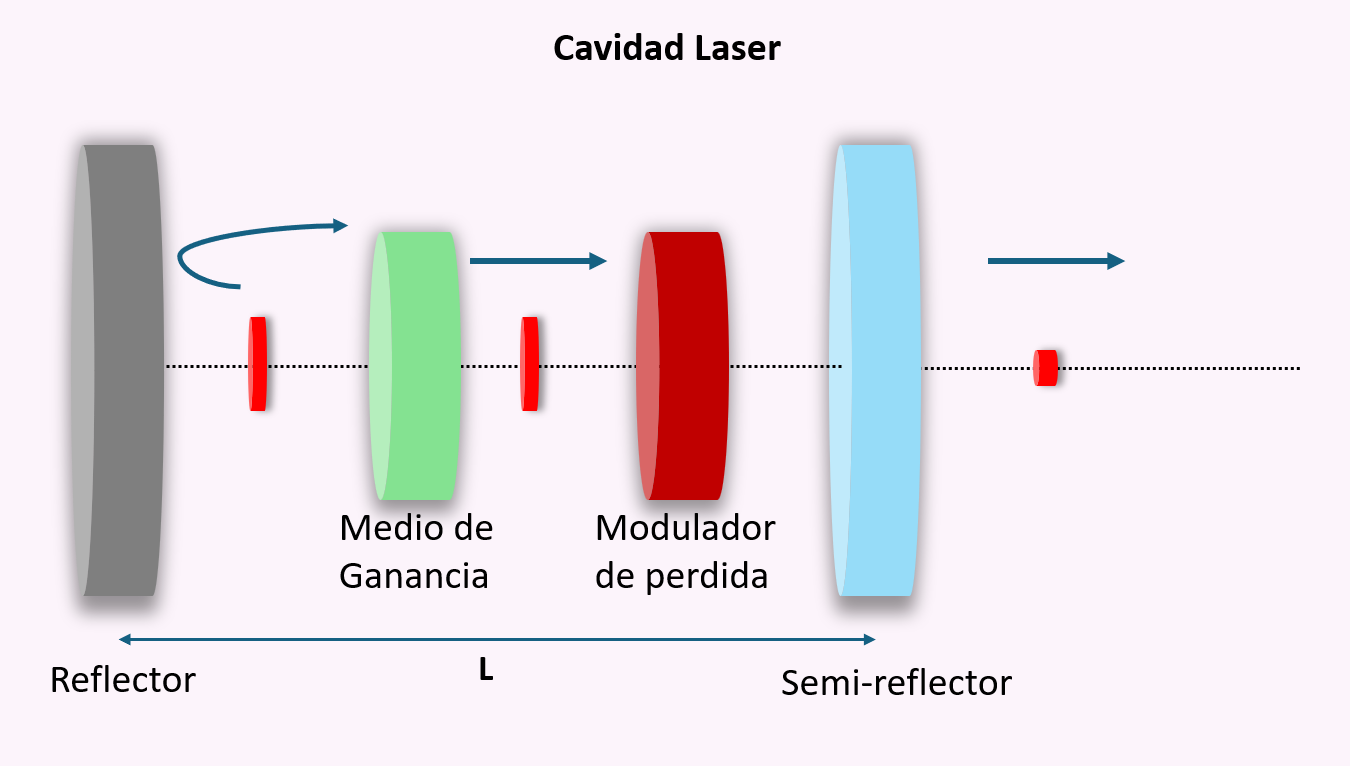
\includegraphics[scale=0.3]{chapters/images/ch3/CavidadLaser_fig3.png}
    \caption{Representación esquemática de la cavidad resonante de un láser de longitud L, diseñada para operar en régimen de bloqueo de modos. El sistema alberga un medio activo (ganancia) y un elemento de modulación (pérdida). La cavidad está delimitada por un espejo de alta reflectancia (HR) en un extremo y un espejo acoplador de salida semitransparente (OC) en el opuesto.}
    \label{fig:CavidadLaser_fig3}
\end{figure}

La arquitectura clásica de un láser de modos bloqueados requiere la integración de un elemento modulador en el interior de la cavidad (véase la Figura \ref{fig:CavidadLaser_fig3}). La propagación del campo electromagnético a través de este componente permite la formación de pulsos sincronizados con los instantes de mínima atenuación impuestos por el modulador. La periodicidad intrínseca de esta modulación coincide con el tiempo de vuelo de ida y vuelta de la cavidad, matemáticamente definido como $T_R=2/Lv_g$, donde $L$ representa la longitud óptica de la cavidad y $v_g$ denota la velocidad de grupo del paquete de ondas en el medio.

\subsection{Procesos inmersos en el bloqueo de modos}

Para establecer y sostener el régimen de bloqueo de modos, es imperativo incorporar un mecanismo (moduladores activos o pasivos fuertemente no lineales) que induzca una relación de fase rígidamente coherente entre los múltiples modos longitudinales resonantes de la cavidad. La dinámica espaciotemporal del pulso ultracorto durante su propagación intracavidad está dictada por una interacción altamente compleja de diversos fenómenos físicos macroscópicos:

    \begin{itemize}
        \item Ganancia. Como en todo oscilador, se requiere un medio activo que provea amplificación suficiente para compensar las pérdidas totales. Mientras que en regímenes monomodo la ganancia es sensible exclusivamente a la potencia promedio, en el bloqueo de modos la elevada intensidad pico de los pulsos ultracortos puede inducir una saturación dinámica y rápida del medio activo (efecto particularmente relevante en láseres de colorante o semiconductores). Este agotamiento abrupto de la ganancia forma asimétricamente el perfil del pulso, facilitando su acortamiento temporal.
        \item Perdida lineal. Engloban la atenuación no dependiente de la intensidad resultante de la transmisión intencionada a través del acoplador de salida, así como la absorción y dispersión parásitas en los componentes ópticos. Un diseño que optimice la relación entre ganancias y pérdidas lineales es insoslayable para suprimir inestabilidades del tipo Q-switching y garantizar la estabilidad macroscópica del tren de pulsos.
        \item Modulación activa. Consiste en la introducción de un elemento acustoóptico o electroóptico (modulador de amplitud o fase) impulsado por un sintetizador de radiofrecuencia externo. Para lograr el bloqueo de modos, la frecuencia de este forzamiento externo debe coincidir con la frecuencia del resonador pasivo, induciendo bandas laterales que acoplan en fase los modos longitudinales adyacentes.
        \item Pérdida saturable (Modulación pasiva de amplitud): Ocurre cuando la atenuación intracavidad responde de manera inversamente proporcional a la intensidad fluente. Este mecanismo no lineal favorece la transmisión de las intensidades pico (reduciendo las pérdidas) y atenúa las componentes de baja intensidad o ruido de fondo. Los dispositivos de pérdida saturable (tales como los Espejos Absorbedores Saturables de Semiconductor o SESAMs, y el efecto de lente de Kerr, KLM) se clasifican en "rápidos" o "lentos" en función del tiempo de relajación de sus portadores relativos a la duración del pulso. Los absorbedores rápidos son excepcionalmente efectivos para regímenes de femtosegundos dado que moldean simétricamente la envolvente del pulso mediante una modulación instantánea.
        \item Modulación de autofase (SPM): Derivada del efecto Kerr óptico, la SPM es un fenómeno paramétrico en el cual el índice de refracción del material depende de la intensidad lumínica transitoria. En osciladores ultrarrápidos, su tiempo de respuesta es cuasi-instantáneo, provocando un desplazamiento de fase no lineal proporcional a la envolvente temporal del pulso, lo que invariablemente se traduce en la generación de nuevas componentes frecuenciales y un severo ensanchamiento espectral.
        \item Dispersión de la velocidad de grupo (GVD): La dependencia de la velocidad de fase con la frecuencia (dispersión cromática) provoca que las distintas componentes espectrales del pulso transiten por la cavidad con velocidades diferenciadas. En un medio de dispersión normal, esto induce un ensanchamiento temporal (chirping) sistemático del pulso. Para contrarrestar esta deformación y preservar la coherencia temporal, es imperativo implementar esquemas de compensación intracavidad (e.g., pares de prismas o espejos fuertemente chirpeados).
        \item Dinámica solitónica: Es el corolario del balance determinista entre la Modulación de autofase (SPM) y una dispersión anómala neta en la cavidad. Mientras la SPM genera un chirp de frecuencia positiva en el frente del pulso, la dispersión anómala invierte este efecto. Su mutua cancelación permite la propagación de "solitones ópticos", paquetes de onda robustos que mantienen una estructura temporal invariante a lo largo de miles de tránsitos intracavidad.
        \item Limitaciones del ancho de banda y filtrado pasivo: La emisión transitable en el oscilador está acotada por el ancho de banda intrínseco del medio de ganancia y la reflectividad espectral de la óptica intracavidad. Por el principio de incertidumbre de tiempo-ancho de banda, el límite de duración temporal mínima de un pulso ultracorto está dictaminado por la máxima anchura espectral que los elementos pasivos permitan oscilar coherentemente, constituyendo el límite fundamental de la técnica.
    \end{itemize}


\subsection{Principios básicos del bloqueo de modos}

La dinámica de oscilación en una cavidad láser está intrínsecamente gobernada por las condiciones de frontera, las cuales definen los modos axiales permitidos. El bloqueo de modos (mode-locking) consiste en el establecimiento de una relación de fase fija y coherente entre estos modos longitudinales. Este fenómeno se induce mediante la incorporación de un mecanismo de modulación intracavidad que genera una perturbación periódica en las pérdidas o en la ganancia del resonador, forzando la oscilación simultánea y sincronizada de múltiples modos. La interferencia constructiva resultante de este acoplamiento de fase da lugar a la formación de pulsos ultracortos de alta intensidad, mientras que la interferencia destructiva en las regiones inter-pulsos minimiza la emisión en el dominio temporal.

\begin{figure}[h]
    \centering
    \begin{minipage}{0.47\textwidth}
        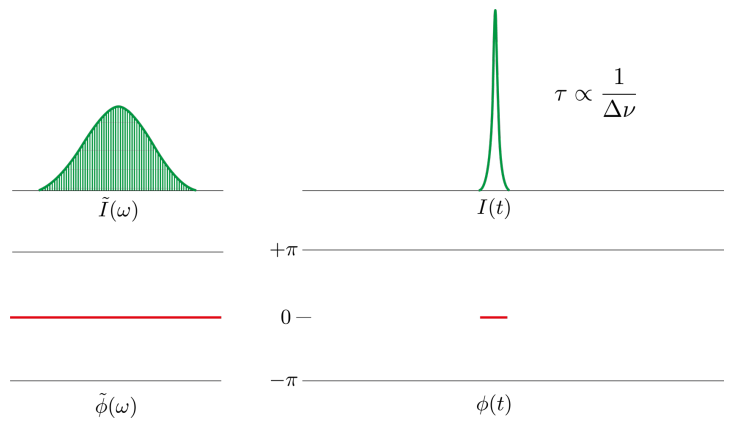
\includegraphics[width=\textwidth]{chapters/images/ch3/Modelocking_fig2a.png}
    \end{minipage}
    \hfill
    \begin{minipage}{0.47\textwidth}
        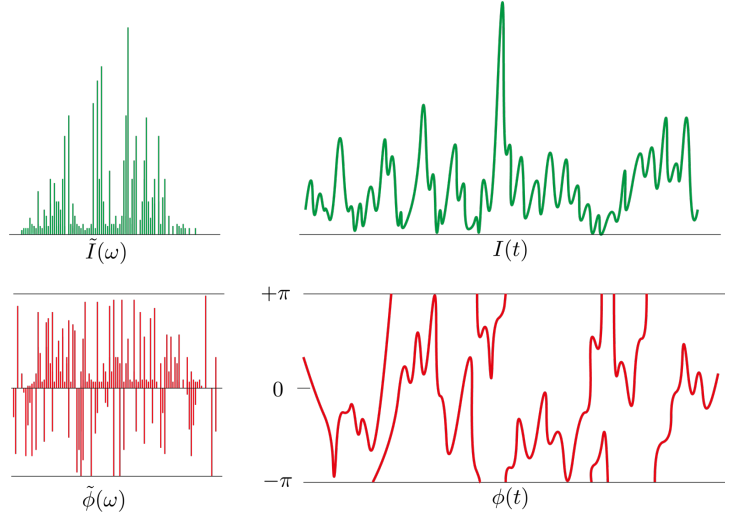
\includegraphics[width=\textwidth]{chapters/images/ch3/Modelocking_fig2b.png}
    \end{minipage}
    \caption{Caracterización del espectro óptico en función de la intensidad $\tilde{I}(\omega)$ y la fase $\tilde{\phi}(\omega)$. a) Régimen de bloqueo de modos (mode-locking): la coherencia de fase entre los múltiples modos longitudinales genera un espectro estructurado y estable, cuya interferencia constructiva resulta en la formación de un pulso ultracorto en el dominio temporal. b) Régimen de emisión multi-modo incoherente: la distribución estocástica de la intensidad y la fase en los modos axiales produce una señal temporal caracterizada por fluctuaciones aleatorias consistentes con ruido óptico, impidiendo la formación de una envolvente de pulso definida .}
    \label{fig:blockMOde&CW}
\end{figure}

La duración del pulso $\tau_p$ es inversamente proporcional al número de modos acoplados, lo que implica que un mayor ancho de banda espectral permite la generación de pulsos temporalmente más estrechos, limitados únicamente por la transformada de Fourier. Para un conjunto de modos axiales con un espaciamiento de frecuencia angular constante $\Delta \omega_{ax}$, una amplitud compleja $\tilde{E}(\omega)$ y una distribución de fase $\phi(\omega)$, el campo eléctrico en el dominio de la frecuencia se expresa como:

\begin{equation}
    \tilde{E}_{tren}(\omega) = \tilde{E}(\omega)e^{i\tilde{\phi}(\omega)} \sum_{m=-\infty}^{\infty} \delta(\omega - m\Delta \omega_{ax})
    \label{eq:6.1}
\end{equation}

donde $m \in \mathbb{Z}$ indexa los modos longitudinales. En el dominio espectral, la intensidad $\tilde{I}_{tren}(\omega) = |\tilde{E}_{tren}(\omega)|^2$ se manifiesta como un peine de frecuencias. Al aplicar la transformada inversa de Fourier a la ecuación \eqref{eq:6.1}, se obtiene la descripción del tren de pulsos en el dominio temporal:

\begin{equation}
    \begin{aligned}
        I_{tren}(t) &= I_p(t) \ast \sum_{m=-\infty}^{\infty}\delta(t - mT_{R})\\
        &= \int_{-\infty}^{\infty} \sum_{m=-\infty}^{\infty}\delta(\tau - mT_{R}) I_p(t - \tau) d\tau\\
        &= \sum_{m=-\infty}^{\infty} \int_{-\infty}^{\infty} \delta(\tau - mT_{R}) I_p(t - \tau) d\tau\\
        &= \sum_{m=-\infty}^{\infty} I_p(t - mT_{R}) 
        \end{aligned}
    \label{eq:6.2}
\end{equation}

donde se ha empleado el hecho de que la transformada de Fourier de un peine de deltas produce otro peine de deltas, y que el producto de dos funciones en el dominio espectral equivale a la convolución de sus transformadas de Fourier inversas. Esta resultado ilustra como el tren de pulsos en el dominio temporal es una suma de pulsos individuales $I_p(t)$, cada uno desplazado temporalmente por un múltiplo entero del período de repetición $T_R$. La duración de cada pulso individual $I_p(t)$ viene dada por $\tau_p$, el cual está determinado por el ancho espectral óptico $\tilde{I}(\nu)$, y una tasa de repetición definida como:

\begin{equation*}
    f_{rep} = \Delta\nu_{ax} = \frac{\Delta\omega_{ax}}{2\pi} = \frac{1}{T_R}.
    \label{eq:tasa_repeticion}
\end{equation*}

Es imperativo distinguir entre la naturaleza espectral de un pulso aislado y la de un tren de pulsos. Mientras que un pulso único presenta un espectro continuo, la periodicidad intrínseca del tren de pulsos impuesta por la cavidad resulta en un espectro discreto o "peine de frecuencias". Como se ilustra en la Figura \ref{fig:blockMOde&CW}, el bloqueo de modos transforma una emisión multi-modo incoherente (ruido) en una estructura temporalmente localizada y altamente estable.

\begin{figure}[h]
    \centering
    \begin{minipage}{0.47\textwidth}
        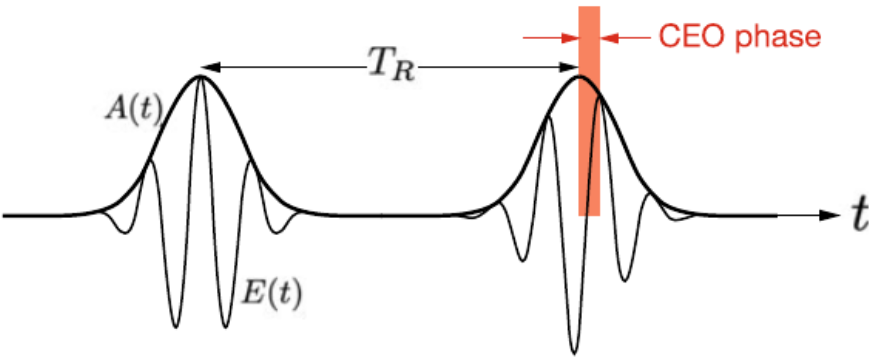
\includegraphics[width=\textwidth]{chapters/images/ch3/CEO_Phase.png}
        \small (a) Dominio temporal.
    \end{minipage}
    \hfill
    \begin{minipage}{0.47\textwidth}
        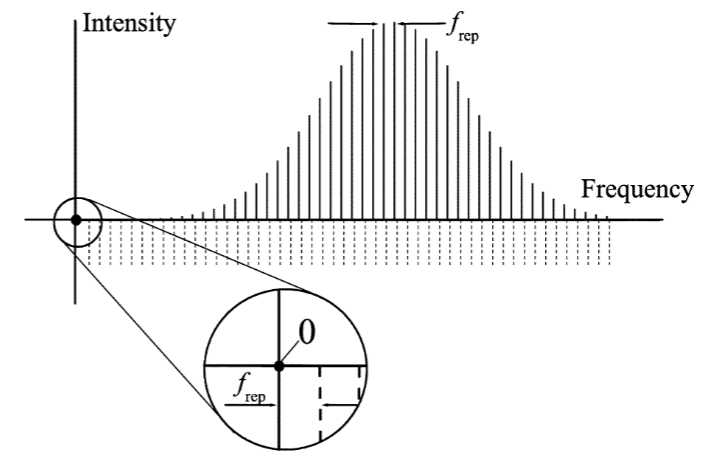
\includegraphics[width=\textwidth]{chapters/images/ch3/equidistantFrecuencyComb.png}
        \small (b) Dominio espectral.
    \end{minipage}
    \caption{
    Dinámica temporal y espectral de un tren de pulsos ultracortos. a) Representación en el dominio temporal donde se ilustra la evolución de la fase portador-envolvente (CEO). La disparidad entre las velocidades de grupo y de fase en la cavidad induce un desplazamiento relativo ($\Delta\phi_{ce}$) del campo eléctrico respecto a la envolvente en cada periodo de repetición $T_R$ \cite{Keller_2022}. b) Representación en el dominio espectral evidenciando la estructura de peine de frecuencias ópticas. El sistema posee dos grados de libertad fundamentales: el intervalo entre modos ($f_{rep} = 1/T_R$) y la frecuencia de compensación portador-envolvente ($f_{CEO}$). En condiciones de dispersión nula, donde las velocidades de fase y grupo coinciden, el campo eléctrico se reproduce idénticamente de pulso a pulso, resultando en un espectro cuyas líneas son múltiplos enteros de $f_{rep}$ ($f_{CEO} = 0$) \cite{keller_2003}.}
    \label{fig:equidistantFrecuencyComb}
\end{figure}

Para la generación de pulsos ultrarrápidos, el láser debe oscilar en tantos modos axiles como sea posible, con una relación de fase constante entre ellas. Diferentes técnicas y métodos existen para establecer esta condición dentro del láser. Todas estas técnicas se denominan "técnicas de bloqueo de modos", por que los modos que forman el peine de frecuencias están bloqueados en fase y tienen una distribución de fase bien definida. Se pueden clasificar en dos categorías principales: bloqueo de modos activo y bloqueo de modos pasivo. El bloqueo de modos activo emplea moduladores externos (acusto-ópticos o electro-ópticos) sincronizados con $T_R$. Por otro lado, el bloqueo de modos pasivo utiliza elementos no lineales, tales como absorbedores saturables (SESAM) o el efecto Kerr óptico, los cuales modulan las pérdidas en función de la intensidad instantánea, permitiendo alcanzar regímenes de femtosegundos

En sistemas de pocos ciclos, cobra importancia un grado de libertad crítico: el desplazamiento de fase portador-envolvente (carrier-envelope phase, CEP). Debido a la dispersión intracavidad, la velocidad de fase y la velocidad de grupo difieren, provocando que el máximo del campo eléctrico se desplace respecto a la envolvente del pulso en cada tránsito. Este fenómeno se traduce en el dominio espectral como un desplazamiento global del peine de frecuencias por una cantidad denominada frecuencia de compensación portador-envolvente, $f_{CEO}$. Así, la frecuencia de cada diente del peine queda definida por $f_m = m f_{rep} + f_{CEO}$, parámetro fundamental en metrología de frecuencias y óptica de campo fuerte.




\section{Solitones}









\section{Bloqueo de modos activo}

El bloqueo de modos activo es una de las primeras técnicas desarrolladas para generar pulsos ultrarrápidos. Consiste en la introducción de un modulador intracavidad, el cual puede ser de tipo acusto-óptico o electro-óptico, que modula periódicamente las pérdidas o la ganancia del resonador. Para lograr el bloqueo de modos, la frecuencia de este forzamiento externo debe coincidir con la frecuencia del resonador pasivo, induciendo bandas laterales que acoplan en fase los modos longitudinales adyacentes. La radiación inicial del láser es reducida una y otra vez en su transito por el modulador, hasta que se alcanza un régimen de oscilación estable donde los modos axiales están acoplados en fase, dando lugar a la formación de pulsos ultracortos. 

\subsection{Pulsos solitónicos en régimen de bloqueo de modos}

Bajo el actuar de ambos GDD y SPM, el régimen de bloqueo de modos puede evolucionar hacia la formación de solitones ópticos, los cuales son paquetes de onda que mantienen su forma temporal invariante a lo largo de la propagación en la cavidad. Este fenómeno ocurre cuando el efecto de modulación de autofase (SPM) induce un chirp positivo en el frente del pulso, mientras que la dispersión anómala produce un chirp negativo, resultando en una mutua cancelación que estabiliza la forma del pulso. Un modulador de pérdida sinusoidal como el ofrecido por un modulador acusto-óptico, no tendrá un efecto muy fuerte sobre la formación del solitón debido a que su duración temporal es mucho más larga que la duración del pulso. 

Los operadores correspondientes a los efectos de SPM y GDD en la ecuación maestra de Haus se pueden expresar como:

\begin{equation}
    \Delta A_4 = -i\delta|A|^2 A(T, t),
    \label{eq:SPM_change}
\end{equation}

mientras que para GDD

\begin{equation}
    \Delta A_5 = iD\frac{\partial^2}{\partial t^2} A(T, t).
    \label{eq:GDD_change}
\end{equation}

De la forma base de la ecuación maestra de Haus (ecuación. (\ref{})), se puede obtener la ecuación maestra para el régimen solitónico de bloqueo de modos activo, la cual se expresa como:

\begin{equation}
    T_R\frac{\partial}{\partial t} A(T, t) = \bigg[iD\frac{\partial^2}{\partial t^2}  - i\delta |A|^2  \bigg] A(T, t)
    + \bigg[g - l + D_g \frac{\partial^2}{\partial t^2} - M(1 - cos(\omega_m t)) \bigg] A(T, t) = 0
    \label{eq:Haus_soliton}
\end{equation}

La primera parte de la ecuación (\ref{eq:Haus_soliton}) es la ecuación de Schrödinger no lineal (ecuación. (\ref{})), cuya solución conocemos para GDD $ < 0$ y $n_2 > 0$ (solitón fundamental). Materiales láser con un ancho de banda de ganancia lo suficientemente grande para generar pulsos ultracortos también cumplirán que $D_g = \frac{g}{\Omega_g^2} \ll 1$. Esto junto el hecho ya comentado de la modulación de pérdida sinusoidal no tendrá un efecto muy fuerte sobre la formación del solitón, nos permite ver que la primera parte de la ecuación (\ref{eq:Haus_soliton}) será dominante en la dinámica del pulso, relegando así el carácter del segundo término a un actor perturbativo. La solución de esta ecuación maestra se halla por  medio de la teoría de perturbaciones solitónicas, en donde la solución con forma Gaussiana es reemplazada por una forma de secante hiperbólica. Los términos debidos a ganancia y pérdida por  modulación pasan a tener un papel fundamental en la estabilización del pulso solitónico, ya que el equilibrio entre ambos es el que determina la energía del pulso.

Un pulso de solitón no se forma de forma instantánea en el resonador. Esto sucede luego que un pulso inicial recorre cierta cantidad de veces por la cavidad y tras estabilizarse resulta en un pulso de solitón. Supongamos un pulso inicial Gaussiano con una duración determinada. Tras miles de recorridos en el resonador, el sistema evoluciona hacia un pulso en estado estacionario con características de solitón, que tiene una duración  mucho menor. Dentro de los primeros 100 recorridos en el resonador, el pulso Gaussiano inicial se convierte en un pulso de solitón. La energía del pulso inicial que no logra ajustarse a la forma del solitón se distribuye en el denominado continuo. El continuo es una parte del pulso con menor intensidad que no puede formar parte del solitón debido a las faltas de balance entre los efectos no lineales y dispersivos. Dado que el continuo tiene una menor intensidad, la SPM es insuficiente para contrarrestar el ensanchamiento temporal causado por la dispersión. Como resultado, el continuo se expande temporalmente. Cuando el continuo se ensancha lo suficiente, experimenta mayores perdidas debido al modulador de perdidas, lo que hace que el continuo disminuya con el tiempo (Fig. (\ref{fig:time_evolution_Nd:YAG})).

En el marco de referencia del solitón, este experimenta un desplazamiento periódico de fase debido al efecto Kerr (referenciar SECCIÓN). Este desplazamiento de fase genera interferencias periódicas entre el solitón y el continuo. Dichas interferencias desaparecerán gradualmente a medida que el continuo decae, dejando únicamente al solitón.

\begin{figure}
    \centering
    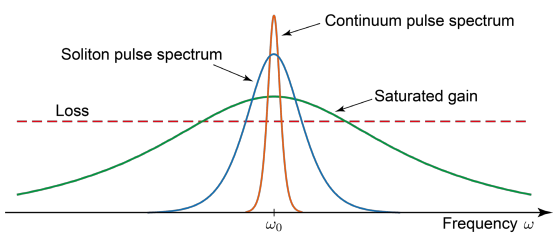
\includegraphics[width=0.8\linewidth]{chapters/images/ch3/saturable_gain.png}
    \caption{La ganancia se satura por el solitón. Sin embargo, ya que el continuo se reduce espectralmente, este verá una mayor ganancia e incremento. La perdida adicional llega únicamente por medio del modulador de perdida, lo cual previene la inestabilidad en el solitón.}
    \label{fig:saturable_gain}
\end{figure}

Para obtener solitones aún más cortos se puede reducir la dispersión del sistema. Sin embargo, una dispersión insuficiente causa que el continuo no se ensanche lo suficientemente rápido para ser absorbido por el modulador de perdidas, lo que lleva a inestabilidades. Después de $10000$ recorridos, estas inestabilidades provocan la formación de los denominados pulsos satélites (pulso más largos y con menor intensidad), que rompen la simetría del pulso propagándose frente al solitón.

Existe un límite en que tanto puede reducirse la duración de los solitones mientras se mantienen estables frente al continuo. Cuando el continuo no decae adecuadamente, el sistema se vuelve inestable y puede generar pulsos adicionales.

El continuo es un pulso residual generado por las perdidas en el modulador, el acoplador de salida y la dispersión del material. Dado que tiene una intensidad mucho menor, no puede mantener el balance entre SPM y la dispersión de grupo negativa (Fig. \ref{fig:saturable_gain})). Este continuo ensanchado eventualmente es suprimido por las mayores perdidas, introduciéndose por el modulador acusto-óptico (Fig. (\ref{fig:GDDbutnoSPMcontinuum})).





\cleardoublepage

\chapter{Metodología}
\label{ch:Methodology}


\cleardoublepage


% \chapter{Resultados}
% \input{chapters/results.tex}
% \cleardoublepage

% \chapter{Discusión}
% \input{chapters/discussion.tex}
% \cleardoublepage

% \chapter{Conclusiones}
% \input{chapters/conclusions.tex}
% \cleardoublepage

% --- Bibliografía ---
% Asegúrate de que el archivo references.bib esté en la raíz del proyecto
% --- Bibliografía ---
\bibliographystyle{unsrtnat}
{
  \raggedright % Alinea a la izquierda y deja el borde derecho irregular
  \bibliography{references}
}

% --- Fin del Documento ---
\end{document}